\chapter{Aspects of quantum chromodynamics}
%in vacuum and at finite temperature}
%%\chapter{Introducing heavy-ion collisions}
\label{chap:pqcd}

\minitoc
\myepigraph{Men of few words require 
  but few laws.}{King X\greek{ar'ilaos}, in \textit{Lycurgus},
  Plutarch}
  % \greek{Ploútar\text{$\chi$}os}}

A lot of work has been carried out over the last century to
explain and understand what are the building blocks of the universe and how they interact. One of the
current undertakings is carried by CERN, the European Organisation for
Nuclear Research, involving theoretical and experimental physicists,
engineers and technical operators altogether.

Among the recent milestones reached in fundamental science, the discovery of the
Higgs boson at the Large Hadron Collider (LHC) is of outstanding importance. It validates the Standard Model of particle physics as the common framework for elementary fermions and bosons, and for three of the four fundamental interactions. 
The new particle indeed appears to be consistent
with massive excitations of the field of the Brout-Englert-Higgs mechanism,
describing the spontaneous breaking of electroweak symmetry $SU(2)
\times U(1)$~\cite{Dawson:1998yi}. This symmetry breaking occurs at an
energy scale within the reach of the proton-proton collisions
performed at the LHC, and the coming years will allow to verify that the new
particle corresponds to the Higgs mechanism, in particular that
all its couplings to known elementary fermions and
bosons are as predicted.

But let us keep the electroweak theory on the side for now and take a step
back. In the past century, our understanding of the interactions
between ``light and matter'' -- now called fermions and bosons -- went
from classical electrodynamics, where it was already known that
any internal symmetry in a closed system translates into a
conservation law, to the Standard Model of particle
physics, benefiting of the advent of quantum field theories (QFT). It
has been understood that, for a \emph{fundamental} physical theory to live in the subnuclear
world, it ought to be:
\begin{itemize}
\item[-] \textit{quantised}, i.e. it should be possible to recast the
  classical fields in quantum mechanical terms, with field operators
  acting on quantum states. Commutation relations between fields
  and/or operators should appear as a result;
\item[-] \textit{locally gauge-invariant}, requiring the physical content
  of the theory to be unchanged by space-time transformations; 
\item[-] as a consequence of gauge invariance, the theory should be
  \textit{symmetric under transformations of the gauge group}, and a
  set of generators define the Lie algebra;
\item[-] \textit{renormalisable}, i.e. the physical modes of
  the newly-formulated quantum theory do not give rise to
  uncancellable divergences when looking at various energy scales;
\item[-] In addition, the theory could be relatively \textit{weakly coupled}; this is a loose
  requirement as we shall see, but a small
  coupling constant allows to compute developments in terms of a perturbation theory.
\end{itemize} 

For electrodynamics and the theory of weak interactions, this has been
achieved with the formulation of the electroweak theory. The degrees
of freedom of this theory are the spin-1/2 particles called fermions
(leptons and quarks), and spin-1 particles called the electroweak bosons
$W^{\pm}$, $\gamma$, $Z^0$. The electroweak theory has the gauge
group $SU(2)_{\rm L} \times U(1)_{\rm hypercharge}$. It is a
renormalisable Yang-Mills theory, as demonstrated in 1972 by the 1999 Nobel-prize winners 't Hooft and Veltman~\cite{tHooft:1972fi}.


Unfortunately, this theory does not explain by itself the stability of nuclei as we know them. Nowadays it is understood that the
cohesion of the nucleus is due to some residual Van-der-Waals
type of force~\cite{longrangeqcd}, as an extension of the pion
exchange first postulated by Yukawa~\cite{yukawa}. But neither does it explain how the inner degrees of freedom are trapped together in a proton, and
why free bare quarks are never directly observed.
% Even
% worse, in the wealth of resonances and particles discovered prior to the
% electroweak bosons, all seem to contain combinations of quarks and
% antiquarks, but some seem to violate the Pauli principle... In
% addition, experiments gradually increasing the energy in the sixties
% and seventies have shown that only a fraction of the proton momentum
% is due to quarks, motivating the quest for an additional set of
% particles, the gluons that bind quarks together... and far more
% surprising, the renormalisability of this new theory of strong
% interactions remained elusive for long, because of the apparition of
% both ultraviolet and infrared divergences...

The coming section is devoted to present several aspects folding
together into quantum chromodynamics, QCD, the gauge theory of the strong
interaction between quarks and gluons.

\section{Building a theory of strong interactions}
\label{sec:strong}
Since the first formulation of neutrons and protons as components of a nuclear
isospin doublet in 1932 by Heisenberg~\cite{heisenberg}, experiments at particle
accelerators have rapidly discovered an increasing number of new particles,
eventually forming a ``particle zoo''. For
about three decades, the dynamics behind this new wealth of unstable particles remained a
puzzle, as every new experiment was discovering a particle, and
additional schematic rules were proposed. Here follows a short chronological review
of what led to formulate $SU(3)_C$ as the group theoretical structure of strong interactions.

\subsection{Nuclear isospin}
\label{sec:isospin}
The proton and neutron have almost equal mass (m$_{n}$ = 939.56~\MeVmass, m$_{p}$ = 938.27~\MeVmass). The proton carries
one positive unit of electric charge, while the neutron is
electrically neutral. At low scattering energies, the experimental
data suggested that the nuclear interaction
$V_{ij}$ is charge independent:

\begin{equation}
V_{pp} \approx V_{pn} \approx V_{nn}
\end{equation}

and the small difference in mass suggested that these two belong to a
single entity, a nuclear isospin $I=\frac{1}{2}$ doublet. Nuclear
isospin is a quantity algebraically equivalent to angular
momentum, but conserved in strong
interactions. In this sense, the new isospin symmetry would be
spontaneously broken (because of the mass degeneracy between the two
components of the $SU(2)$ doublet). This formulation proved practical to establish a list of
isospin multiplets, corresponding to the first discovered hadrons. 
Indeed, from an isospin mutliplet \ket{I,I_{3}} one can construct
2$I$+1 states, including for example the pions and
$\Delta$ resonances:
%\begin{linenomath}
\begin{eqnarray*}
    &\eta = \ket{0,0} \\
    \\
    &p = \ket{\frac{1}{2},\frac{1}{2}} \hspace{1cm} n =
    \ket{\frac{1}{2},-\frac{1}{2}} \\
    \\
    &\pi^{+} = \ket{1,1} \hspace{1cm} \pi^{0} = \ket{1,0} \hspace{1cm}
    \pi^{-}=\ket{1,-1}\\
    \\
    &\Delta^{++}=\ket{\frac{3}{2},\frac{3}{2}} \hspace{1cm} \Delta^{+} =
    \ket{\frac{3}{2},\frac{1}{2}} \hspace{1cm} \Delta^{0} =
    \ket{\frac{3}{2},-\frac{1}{2}} \hspace{1cm} \Delta^{-} =
    \ket{\frac{3}{2},-\frac{3}{2}}  
\end{eqnarray*}
%\end{linenomath}
The study of the $\Delta$ resonances, located at masses around 1232~\MeVmass, helped validating such a model for some time.

\subsection{The Eightfold way, strangeness, and SU(3) flavour
  symmetry}
\label{sec:eightfold}
In the fifties, the kaon family ($K^{\pm}, K^0$) and the Lambda baryon discovery in cosmic rays led to an addition to the isospin
model. These particles were found to be long-lived, produced in pairs
with strict rules: for instance a $\Lambda$ can be produced with a $K^{+}$, but never with a $K^{-}$. So it was advocated that a new quantum number was needed,
\textit{strangeness} $S$, that would be conserved in production occurring from the
strong interaction. This way, the $K^{+}(S=+1)$ produced in addition
with $\Lambda(S=-1)$ was indeed favoured.

A generalised theory of nuclear isospin was underway. As
mentioned above, the isospin multiplets of $\pi$, nucleons and
$\Delta$ would conform to a theoretical group classification with
three generators $I_{\pm},I_3$, making $SU(2)$ a proper group for the
isospin symmetry. With the advent of strangeness, Gell-Mann and
Ne'eman independently put forth a $SU(3)$ model with three flavours
($u$,$d$,$s$)~\cite{eightfoldway,neeman}. Gell-Mann suggested that the
current meson ($q\bar{q}$) and baryon ($qqq$) spectroscopies could be
understood in terms of irreducible representations of the new $SU(3)_F$ flavour group. For objects with integer
electric charge, the first representations contained one, eight, ten
members. For fractional electric charge objects, a triplet and a
sextet were envisioned, but no particles with fractional charge were
found. People at that time did not take the existence of fractional
electric charges seriously, and the fractional charge triplet (later
known as the $u$, $d$ and $s$ \textit{quarks}) was regarded as a
mathematical artifact, since the electric charge and the baryon
number must be conserved. 

Adding strangeness to the number of flavours led to the
Gell-Mann--Nishijima empirical relation between electric charge $Q$,
baryon number $B$, strangeness $S$ and isospin $I_3$:
\begin{equation}
Q = I_3 + \frac{1}{2}(B + S) 
\end{equation}
where: 
\begin{equation}
I_3 = \frac{1}{2}[(n_{\rm u} - n_{\rm \bar{u}}) - (n_{\rm d} - n_{\rm
  \bar{d}})],
\end{equation}
\begin{equation}
S = -(n_{\rm s} - n_{\rm \bar{s}}), 
\end{equation}
and the baryon number\footnote{This definition
is nowadays extended to include all six quark flavours.} $B$ of a
hadron is here defined as the sum of the
contained net quarks:
\begin{equation}
B = \frac{1}{3}[(n_{\rm u} - n_{\rm \bar{u}}) + (n_{\rm d} - n_{\rm
  \bar{d}}) + (n_{\rm s} - n_{\rm \bar{s}}) ].
\end{equation}

The electric charge $Q$ would then equal to the following, exhibiting
somewhat unforeseen fractional electric charges for each
(not-yet-quark) flavour:
\begin{equation}
Q = \frac{2}{3}(n_{\rm u} - n_{\rm \bar{u}}) - \frac{1}{3}[(n_{\rm d} - n_{\rm
  \bar{d}})+(n_{\rm s} - n_{\rm \bar{s}})]
\end{equation}

 Both mesons and baryons would turn out to fit in the octet
description mentioned above, leading Gell-Mann to coin this model the
\textit{eightfold way}~\cite{eightfoldway}, in a reference to the
Eightfold Path of
Buddhism\footnote{\href{https://en.wikipedia.org/wiki/Noble_Eightfold_Path}{Noble
    Eightfold Path, Wikipedia: https://en.wikipedia.org/wiki/Noble\_Eightfold\_Path}}. A pictorial
representation of the meson octets is presented in
Figure~\ref{fig:mesonoctet}. In each representation, the meson family members share the
same spin-parity: On the left, the ($J^P = 0^-$) pseudo-scalar meson
family is outlayed, and the vector mesons ($J^P = 1^-$) are shown on
the right.

\begin{figure}[h]
\begin{center}
  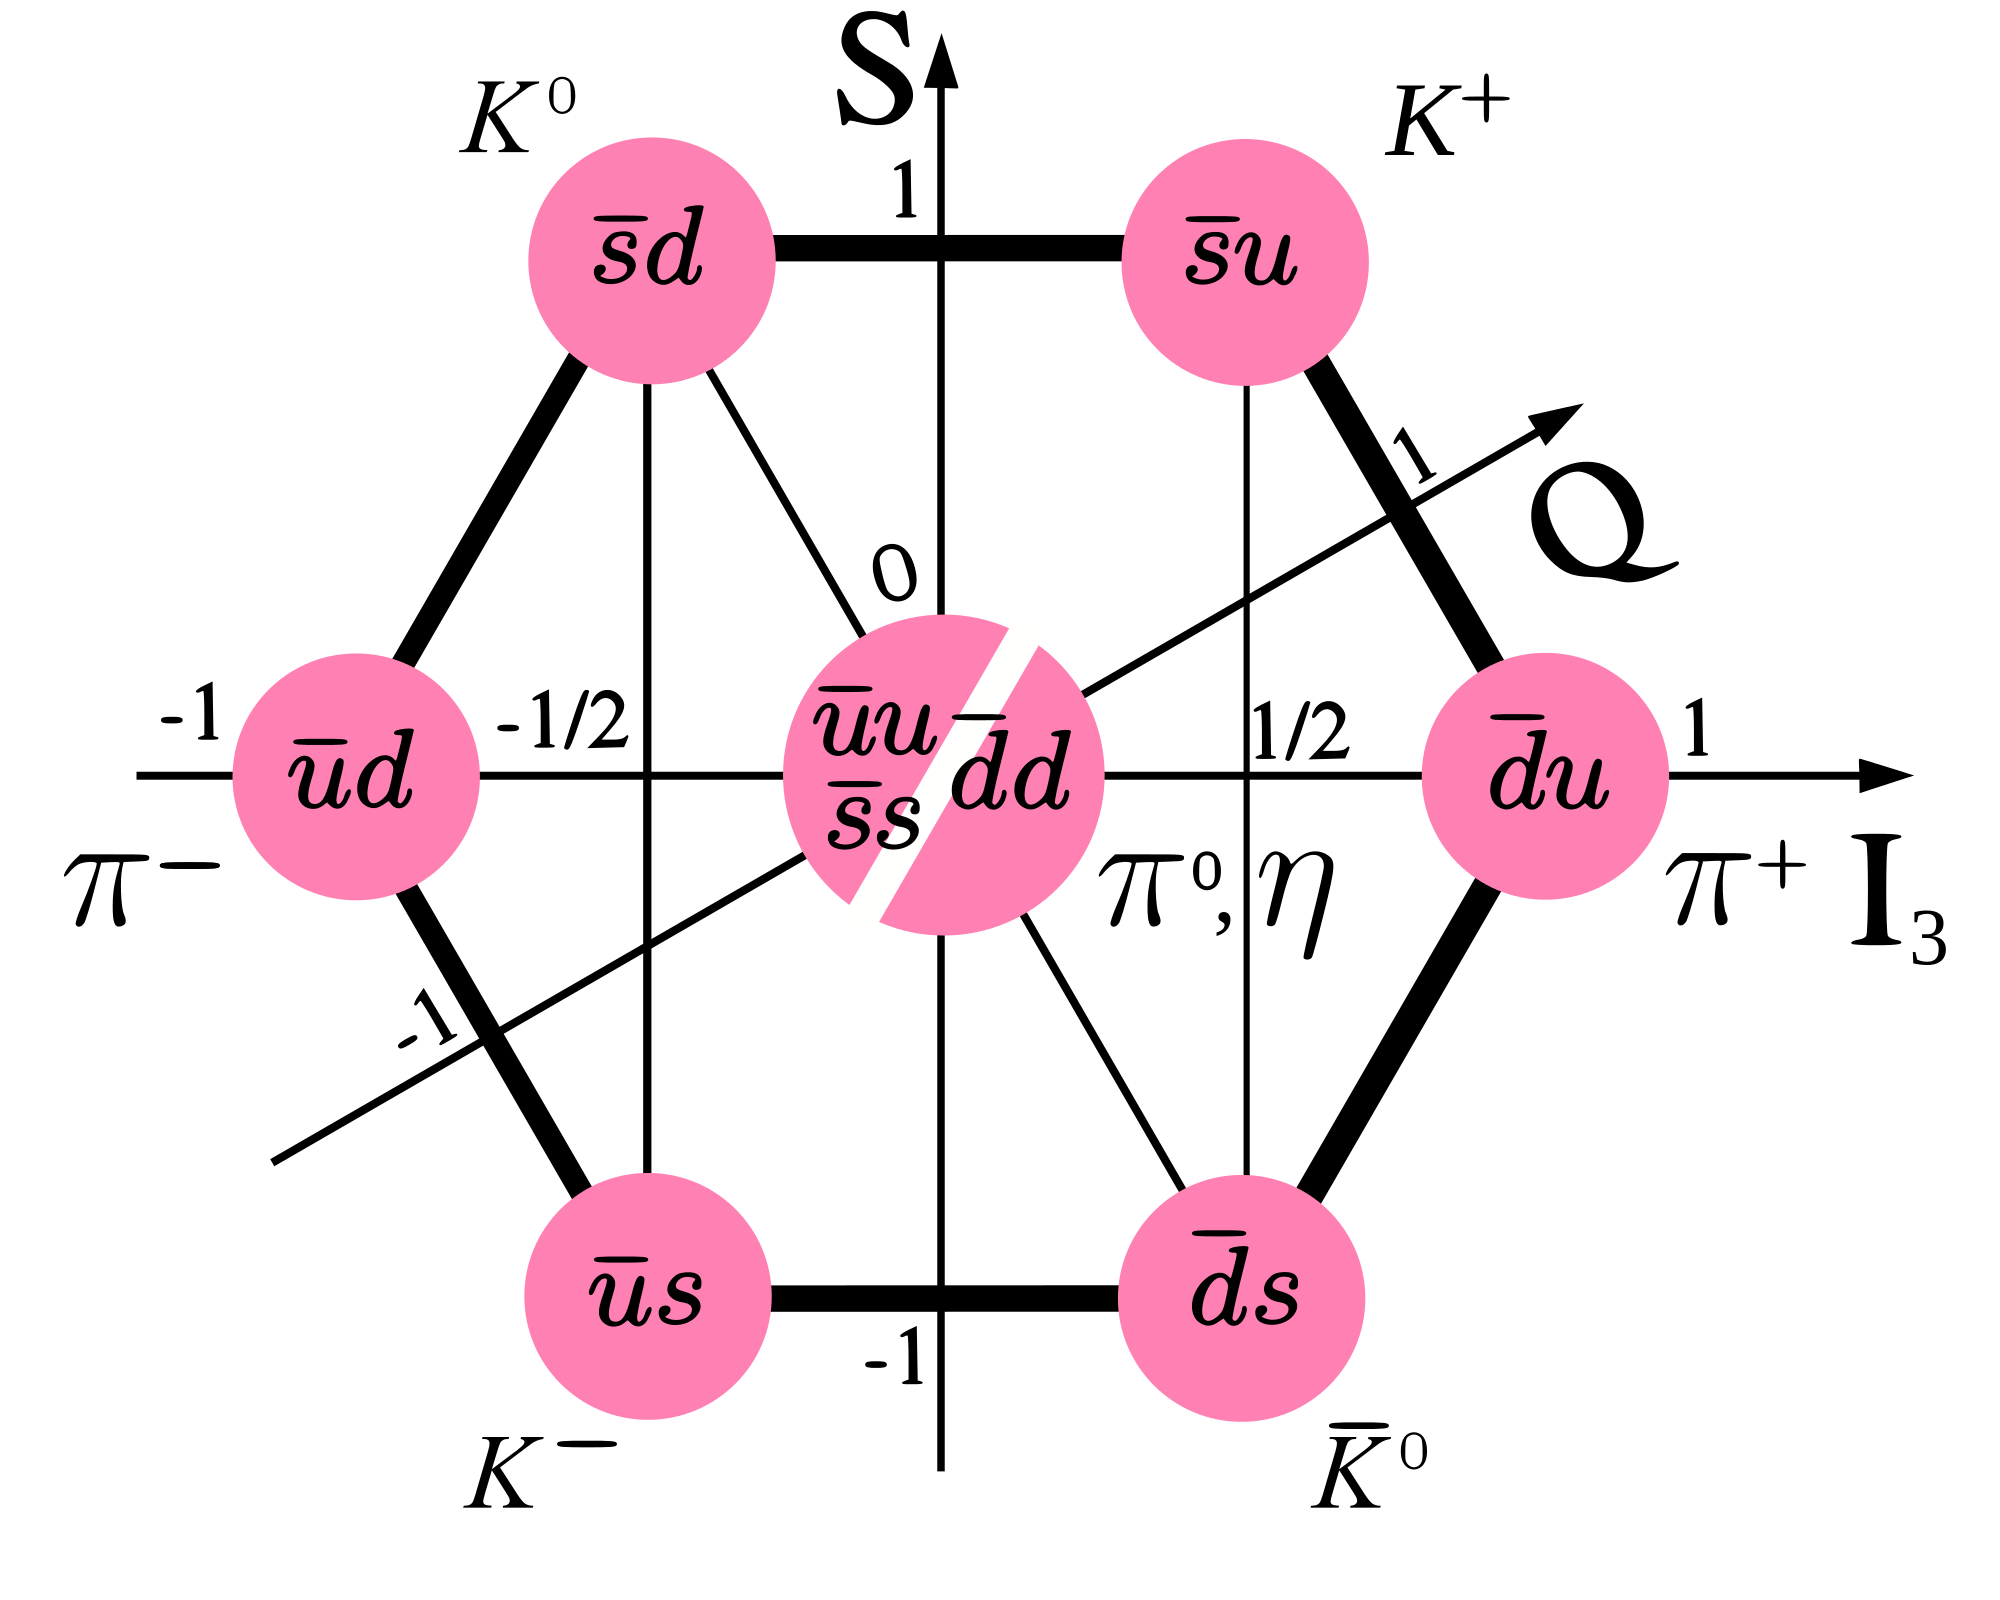
\includegraphics[width=0.45\textwidth]{Chapters/pQCD/Meson-octet_0.png}
  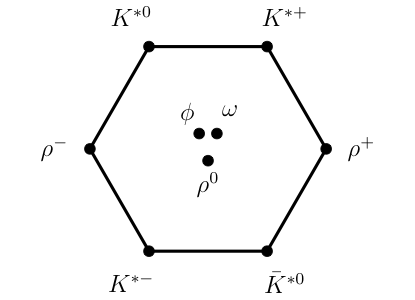
\includegraphics[width=0.45\textwidth]{Chapters/pQCD/Meson-octet_1.png}
 \caption{Left: the pseudo-scalar meson octet. Right: the vector meson octet.}
 \label{fig:mesonoctet}
\end{center}
\end{figure}

As a consequence of the octet structure, Gell-Mann went on to predict in the same paper the existence of
an electrically neutral meson completing the pseudo-scalar meson octet. The $\eta$~meson
was discovered in 1961 by Pevsner and others~\cite{PhysRevLett.7.421}. 

Gell-Mann also pointed out in a 1962 conference that nine known excited
baryons of spin-parity $J^P = 3/2^{+}$ would fit nicely into a decuplet representation of
$SU(3)$ if a tenth baryon carrying strangeness $S=-3$ were to be
found~\cite{1962_GM_omega}. The discovery of the $\Omega^{-}$ baryon in 1964 at
Brookhaven~\cite{omegabaryon} at precisely the mass given by the
theory estimation~\cite{GM_omega,Okubo} sealed the success of the
$SU(3)_F$ flavour symmetry. The complete baryon $J^P = 1/2^{+}$ octet
and $J^P = 3/2^{+}$ decuplet are presented in Figure~\ref{fig:baryonoctet}.

\begin{figure}[h]
\begin{center}
  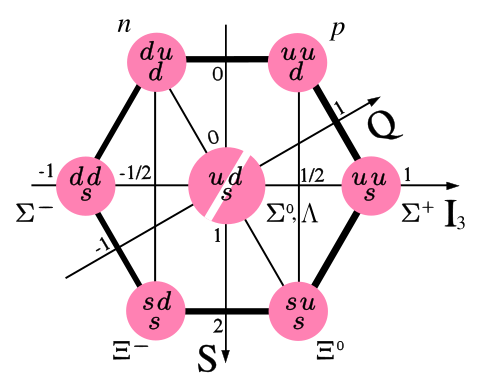
\includegraphics[width=0.45\textwidth]{Chapters/pQCD/Baryon-octet.png}
  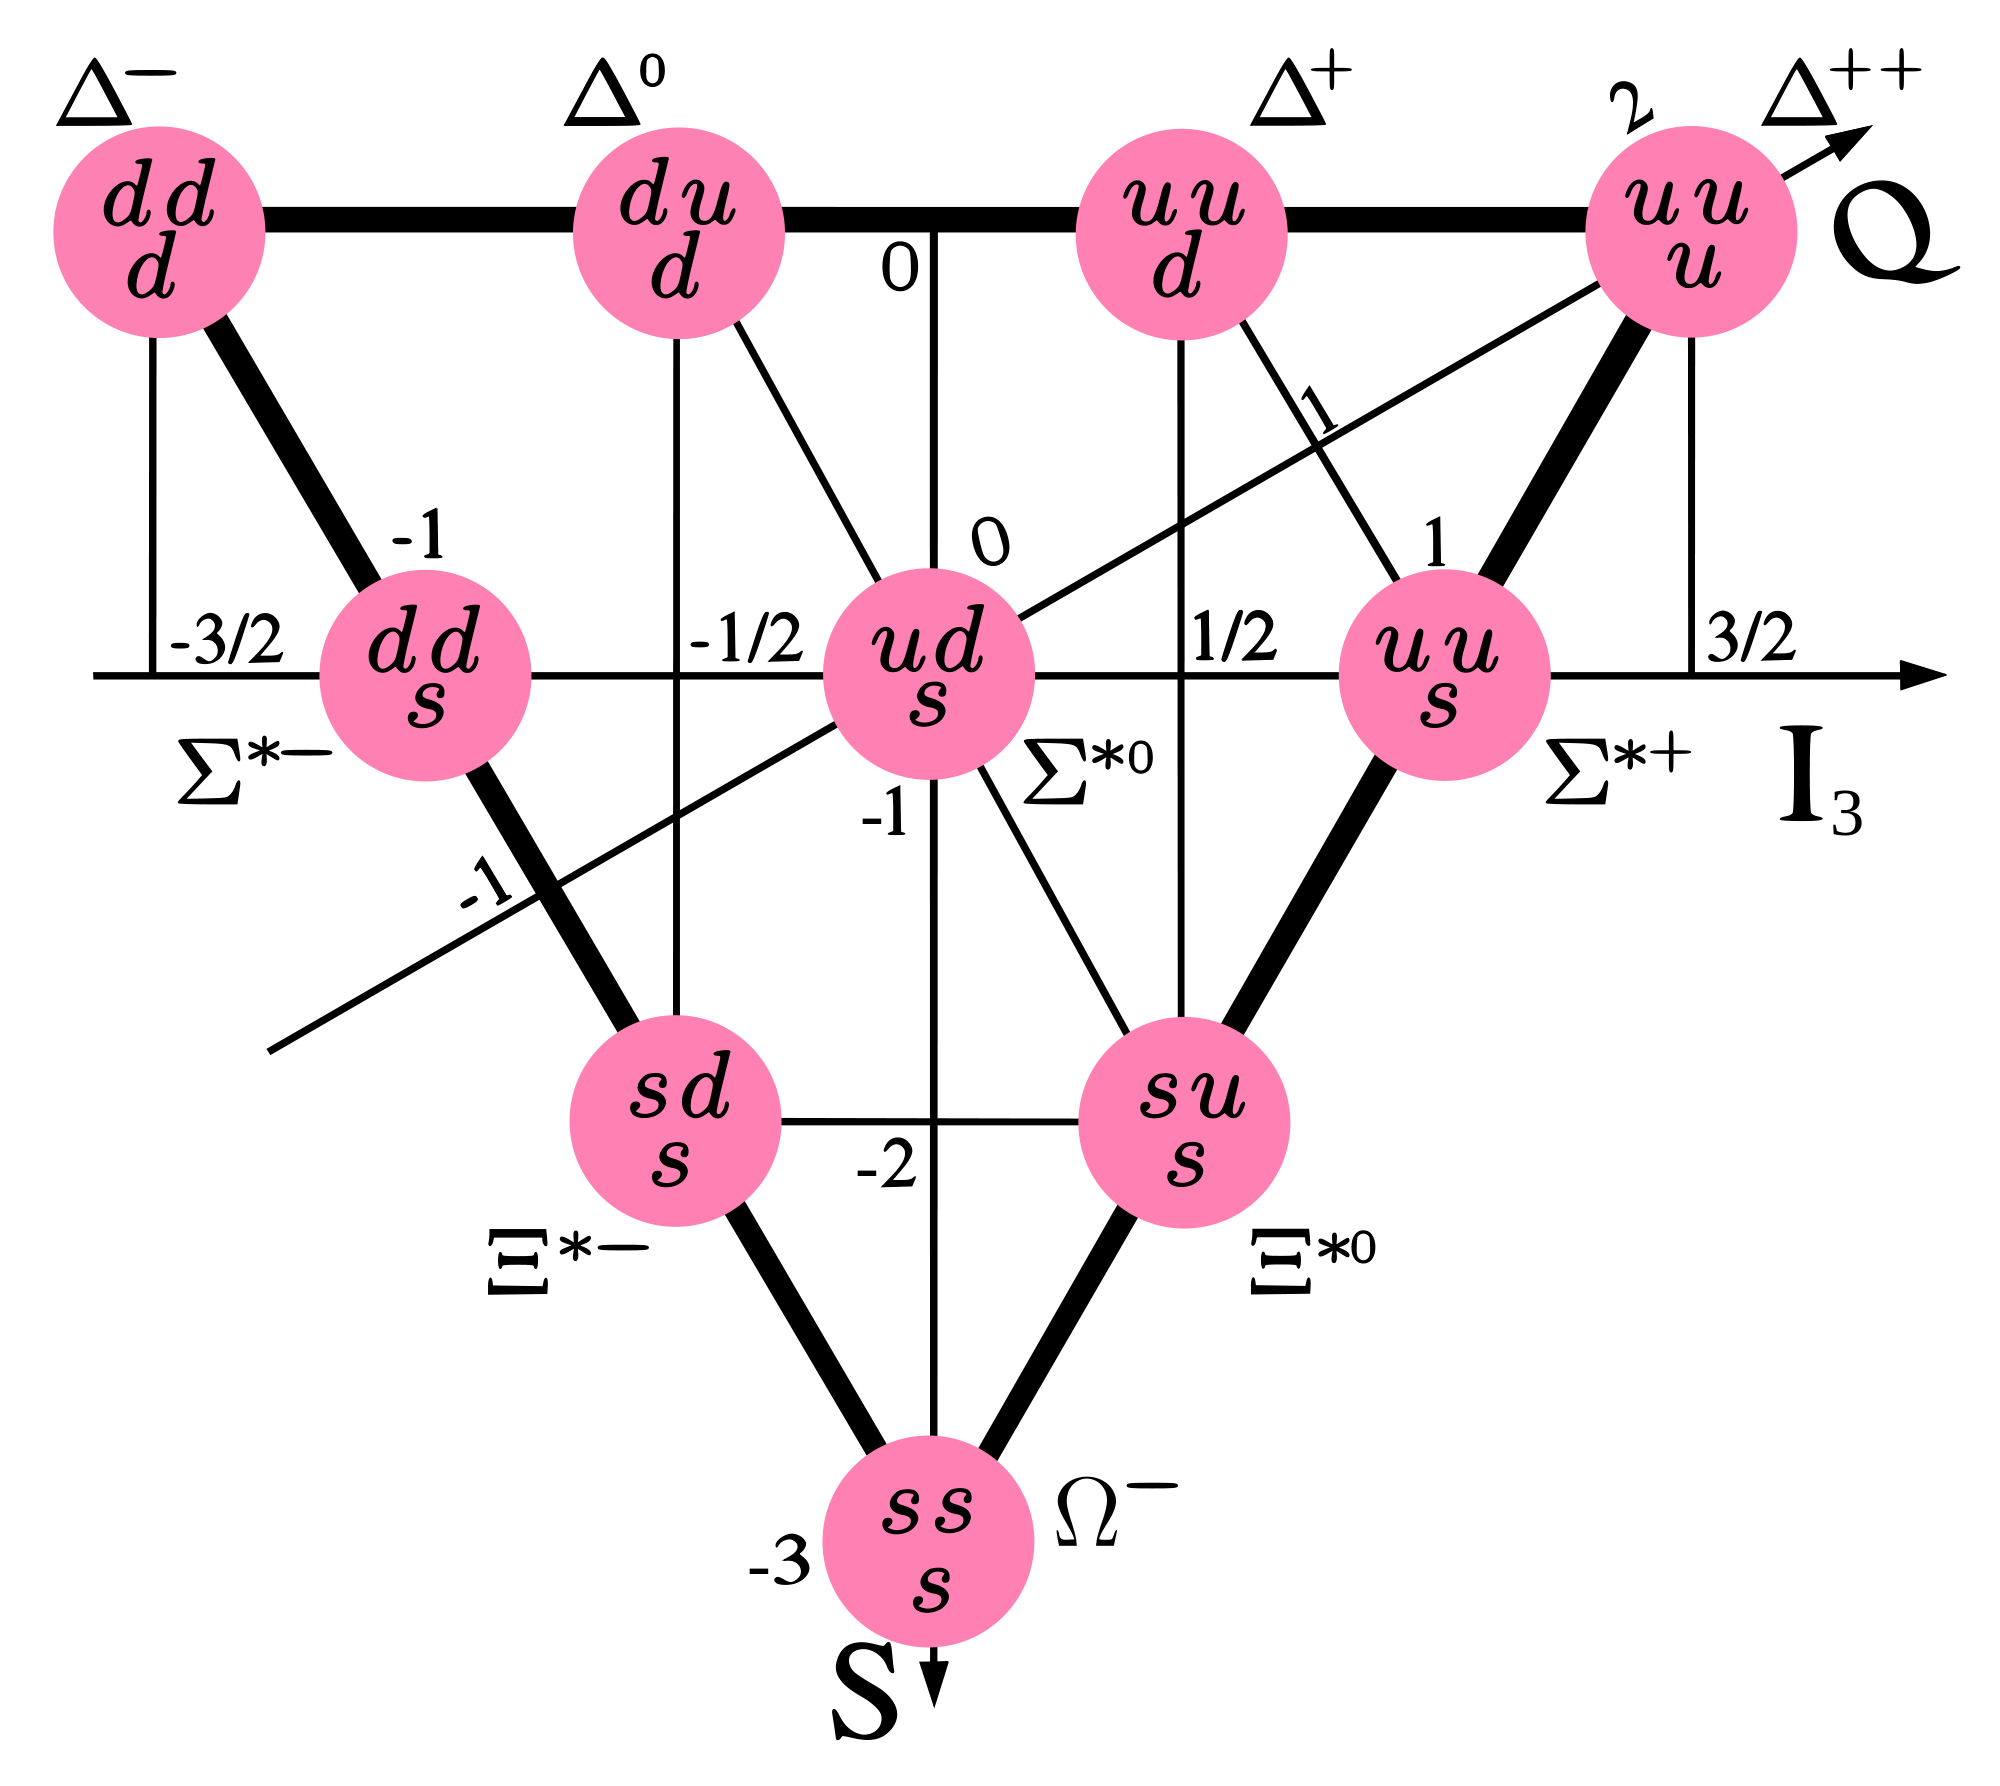
\includegraphics[width=0.4\textwidth]{Chapters/pQCD/Baryon-decuplet.png}
 \caption{Left: the $J^P = 1/2^{+}$ baryon octet. Right: the $J^P =
   3/2^{+}$ baryon decuplet, showing the $S=-3$ baryon $\Omega^-$ at
   the bottom of the decuplet.%  (Note: the change of convention
   % for the orientation of the strangeness axis between left is arbitrary.)
 }
 \label{fig:baryonoctet}
\end{center}
\end{figure}

\subsection{The need for colour}
\label{sec:colour}
By 1964, the static picture of hadrons had emerged. There was an
understanding in the community that a theory of strong interactions
of non-abelian nature
% (likely spontaneously broken, because of the
% differences in masses of the hadrons) 
is underlying, but its dynamics
was yet unknown. What is the force carrier behind the strong
interaction? Where is the triplet of particles of the fundamental
representation of $SU(3)$? These questions would be answered in the
coming ten years with the formulation of the quark model, the parton
picture and
eventually that of QCD.

What I have described here is already a quark
model\footnote{Sometimes, the (u,d,s) model is referred to as
  the 'naive' quark model.}, with three
flavours. Because the masses are not all equal between the
three quark flavours, we can only consider the flavour symmetry as
approximate. % I would like to raise two other problems with the quark model as
% it stands at this point:
% One big problem in the hadron spectroscopy comes from the statistics
% obeyed by the
%. Indeed, according to the

Furthermore, hadron spectroscopy seems to be driven by the wrong
statistics. Indeed, according to spin-parity of the baryon decuplet,
$J^{P} = \frac{3}{2}^{+}$, the baryon wave functions should be fully antisymmetric. Let us consider
the states $\Omega^{-}, \Delta^{++}$ and $\Delta^{-}$ at the
corners of the decuplet diagram (cf. Figure~\ref{fig:baryonoctet} right):
\begin{align*}
&\ket{\Delta^{++}(S_{z}=3/2)} \sim \ket{u^\uparrow u^\uparrow
  u^\uparrow},\\
&\ket{\Delta^{-}(S_{z}=3/2)} \sim \ket{d^\uparrow d^\uparrow
  d^\uparrow},\\
&\ket{\Omega^{-}(S_{z}=3/2)} \sim \ket{s^\uparrow s^\uparrow s^\uparrow}
\end{align*}
We see that each state has three identical spin-aligned quarks. Furthermore, the
decuplet states are at the fundamental level ($L=0$), and all relative
angular momenta between quarks equal to zero. This leads to a fully
symmetric wave function and therefore the three
states obey the wrong statistics. In other words, Pauli's exclusion principle should preclude these particle from existing. 

To anti-symmetrise the baryon states, one can introduce an additional
quantum number, \textit{colour}, such that in this picture, a sum of
permutations of the colour states are contributing to the observed
baryon. In the case of $\Delta^{++}$, one has:
\begin{equation}
\ket{\Delta^{++}} \sim \frac{1}{\sqrt{6}}\epsilon^{\alpha\beta\gamma}\ket{u_{\alpha}^\uparrow u_{\beta}^\uparrow
  u_{\gamma}^\uparrow},
\end{equation}
Where the sum is implicit (using Einstein's convention) over
colours, and $\epsilon^{\alpha\beta\gamma}$ is the fully
anti-symmetric Levi-Civita tensor. One sees that at least three
colours are needed to have an antisymmetric state. In this
description one can construct 9 different colour combinations for the
$q\bar{q}$ meson wave functions, out of which only 3 seem to exist. 
Also, the fact that only $q\bar{q}$ and $qqq$ states are observed is 
a puzzle. 

These two problems are solved by the ad-hoc colour
\textit{confinement hypothesis} that should have a dynamical nature:
since quarks carry colour and hadrons are colour-singlet 
states, there must be a mechanism responsible for equilibrating the
colour content in the final state. Nowadays the colours used for
quarks are
\color{red}\textbf{red}\color{black},~\color{green}\textbf{green}
\color{black}and 
\color{blue}\textbf{blue}\color{black}, while
anti-\color{red}\textbf{red}\color{black},~anti-\color{green}\textbf{green} \color{black} and
anti-\color{blue}\textbf{blue}\color{black}~are antiquark colours. The
choice is of course arbitrary, but inspired by the analogy of
colour-singlet states appearing white.

\subsection{Evidence for quarks}
\label{sec:quarks}
The quark picture put forth in the early sixties did not get
firm approval in the community immediately. Quarks were lacking an
experimental evidence, and it was by no means clear that experiments
would ever be able to produce fractional electric charge particles. The
evidence came from a series of deeply inelastic electron-nucleon
scattering experiments performed
by the SLAC-MIT collaboration (for which Friedman, Kendall and Taylor were awarded the Nobel Prize in Physics in 1990).


The impact of deep inelastic scattering experiments on the inception
of chromodynamics is considerable, and the basics are
presented here. Let us consider the typical reaction $e^{-}+p \to e^{-}+X$ where X is
any number of hadronic remnants in the final state. The diagram in Figure~\ref{fig:dis_test} lays out the kinematics
of the reaction.
\begin{figure}[h]
\begin{center}
  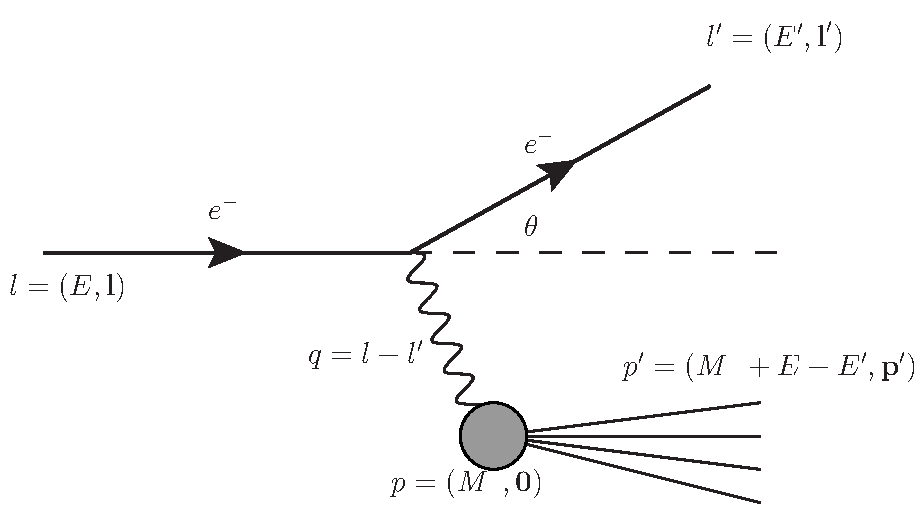
\includegraphics[width=0.7\textwidth]{Chapters/pQCD/DIS_test.pdf}
 \caption{Deep inelastic $e^{-}p$ scattering. A photon is exchanged
   and a hadronic final state X is formed.}
 \label{fig:dis_test}
\end{center}
\end{figure}

The initial high-energy electron scatters off a proton of mass $M$
and four momentum $p$, via the exchange of a space-like virtual
photon. In the final state, $\theta$ is the electron scattering angle, the electron has a
four-momentum $l'$ and the hadronic system has invariant mass $W$. The
energy transfer between the electron and the hadronic system is $\nu$:

\begin{equation}
\nu = E - E' = \frac{q\cdot p}{M}
\end{equation}

and the virtuality of the photon, i.e. its squared momentum transfer
$Q^{2}$ is defined as:
\begin{equation}
Q^{2} = -(l - l^{'})^{2} = 2M\nu + M^{2} - W^{2} \leq
2M\nu .
\label{eq:qsquare}
\end{equation}
In the elastic scattering, where $X$ is made of the initial scattered proton, the rightmost terms of Equation~\ref{eq:qsquare} would turn into an equality.
We can now introduce the so called Bjorken-$x$, $x_{B}$, that would represent how much the
process deviates from the elastic scattering
\begin{equation}
x_{B} = \frac{Q^{2}}{2M\nu}, \hspace{1cm} 0 \leq x_{B} \leq 1.
\end{equation}

 In this sense, when the momentum exchange is negligible, the
final-state invariant mass $W$ tends to $M$, and $x_{B} = 1$
(elastic scattering). In turn, small values of $x_{B}$ correspond to
high momentum exchange, $Q^{2} \gg M \nu$. To test if a target proton contains inner degrees of
freedom, one can consider the cross-section for scattering of a lepton
off a spin-1/2 fermion of mass $M$, charge e$_q$ and specific to
the case of non pointlike particles\footnote{A textbook example of
  this calculation is available for example in Appendix F of~\cite{qcd_book}.}. A double-differential cross
section can be derived as a function of two \emph{structure functions} $W_1$ and $W_2$~\cite{qcd_book}:
\begin{equation}
\frac{d^{2}\sigma}{dQ^{2}d\nu} = \frac{4\pi\alpha^{2}_{QED}}{Q^{4}}\frac{E'}{E}\left( W_2(Q^{2},\nu)\rm{cos}^2\frac{\theta}{2} +
    2W_1(Q^{2},\nu)\rm{sin}^2\frac{\theta}{2} \right)
\label{eq:QED_DIScrosssection}
\end{equation}

In Equation~\ref{eq:QED_DIScrosssection}, the scattering process occurs
via the exchange of a photon, hence the QED coupling constant
$\alpha_{QED}$. Equation~\ref{eq:QED_DIScrosssection} assumes the hypothesis that a nucleon is an extended particle,
composed of several pointlike particles with electric charge $e_i$. One then defines \emph{parton
distribution functions} (PDF) $f_i(x_i)$, representing the probability
that the struck
\textit{parton} carries a momentum fraction $x_i$ of the
nucleon. Thus, the structure constants built with the
parton distribution functions are: 
\begin{equation}
W_1(Q^2,\nu)=\displaystyle\sum_{i}e^{2}_{i}f_{i}(x_{B})\frac{1}{2M}
\end{equation}
and
\begin{equation}
W_2(Q^2,\nu)=\displaystyle\sum_{i}e^{2}_{i}f_{i}(x_{B})\frac{x_{B}}{\nu}.
\end{equation}
One can absorb $M$ and $\nu$ into these definitions to parameterize the lepton-nucleon cross section in deep inelastic scattering (DIS) with two functions that depend only on how the momentum is shared between the nucleon constituents:
\begin{equation}
F_1\equiv M_{h} W_1
=\frac{1}{2}\displaystyle\sum_{i}e^{2}_{i}f_{i}(x), \hspace{1cm}
F_2\equiv \nu W_2 =\displaystyle\sum_{i}e^{2}_{i}xf_{i}(x).
\end{equation}

The fact that DIS processes depend only on $x$, a dimensionless
parameter, translates into the independence of the structure function
F$_2$ with the Q$^{2}$ of the reaction. This is called \textit{Bjorken
  scaling}, and is the main feature of the parton
model~\cite{webber3}. This scaling behaviour was first measured by the
MIT-SLAC collaboration in 1970. Figure~\ref{fig:F2scaling} shows the
$F_{2}$ structure function, as a function of $x$, for various 
DIS energies on a proton target. The scaling here manifests itself in
the form of this universal curve holding for very different values of
$Q^{2}$. This is a definite proof of the existence of pointlike
consituents at these energy scales, as the presence of non-pointlike
particles would make structure functions depend on  $Q/Q_{0}$, with
$1/Q_{0}$ the typical size of the non-pointlike object.

\begin{figure}[h]
\begin{center}
  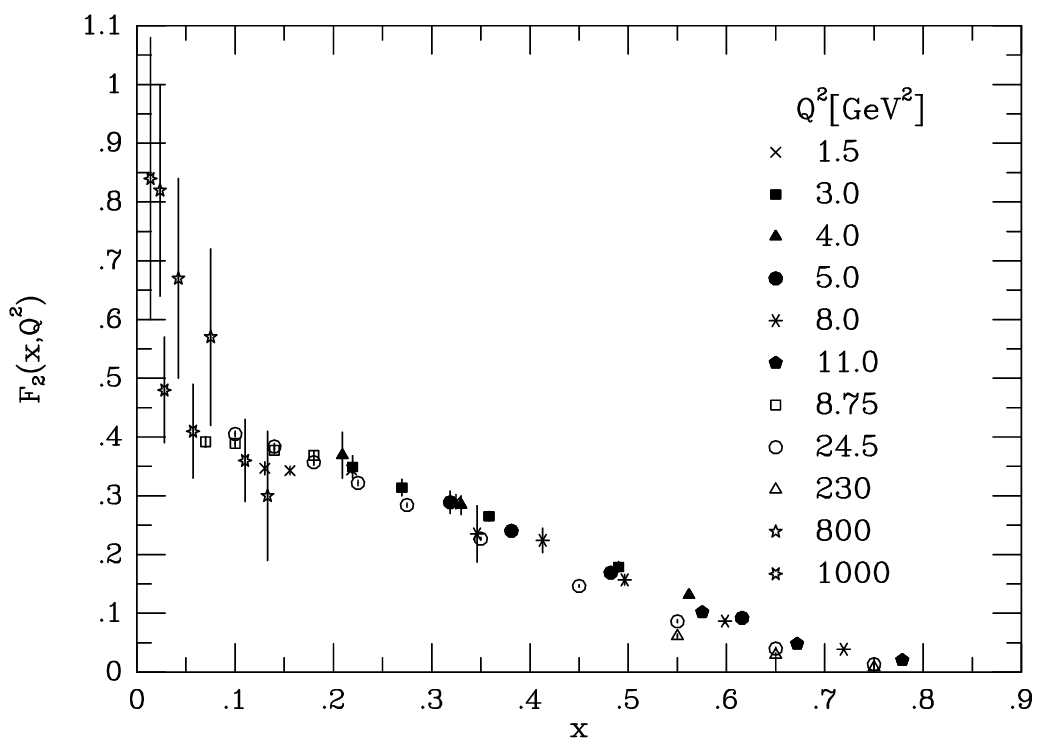
\includegraphics[width=0.7\textwidth]{Chapters/pQCD/F2scaling.png}
 \caption{Structure function $F_{2}$ as a function of $x$. Emergence
   of scaling at various $Q^{2}$ energies in proton DIS. Compilation
   of PETRA data taken from~\cite{webber3}.}
 \label{fig:F2scaling}
\end{center}
\end{figure}

\subsection{On the verge of a revolution}
\label{sec:verge}
I have presented the inherent colour in the quark model, and how
quarks have been discovered in early DIS experiments% , leading to a
% partonic picture of the quark model
. There are many
aspects of the puzzle of this pre-QCD era which 
have not been dealt with. For example, I did not mention that structure
functions can be expressed in terms of the quark -- and anti-quark --
densities inside the target hadron. For example for $u$ and $d$ quarks one
has:
\begin{equation}
u= u_{\rm p}(x) \hspace{0.5cm}d= d_{\rm p}(x) \hspace{0.5cm}\bar{u}= \bar{u}_{\rm p}(x) \hspace{0.5cm}\bar{d}= \bar{d}_{\rm p}(x) \hspace{0.5cm}
\end{equation}

In this sense, doing a DIS experiment allows one to measure the PDFs of
each quark flavour. In the case of electron-deuterium scattering for example, one can
write the two $F_2(x)$ of electron-proton and electron-neutron processes:
\begin{eqnarray}
F_{2}^{ep}(x) &=& x\left[ \frac{4}{9}(u+\bar{u}) + \frac{1}{9}(d+\bar{d}) \right]\\
F_{2}^{en}(x) &=& x\left[ \frac{1}{9}(u+\bar{u}) + \frac{4}{9}(d+\bar{d}) \right].
\end{eqnarray}

These two can be averaged\footnote{The average in any nucleus is
  $F_{2}^{eA}(x) = Z F_{2}^{ep}(x) + (A-Z) F_{2}^{en}(x)$.} to compute
the $F_{2}^{eN}$ of the deuteron:
\begin{equation}
F_{2}^{eN}(x) = \frac{5}{18}x\left(u  + \bar{u} + d + \bar{d}  \right).
\end{equation}
Implicitly, each parton distribution contains a contribution from the three
\textit{valence} quarks of a nucleon, as well as \textit{sea} quarks
and anti-quarks coming from vacuum excitations. It follows that integrating over $x$
should give the total fraction of momentum carried by quark degrees of
freedom. One finds experimentally:

\begin{equation}
\int^{1}_{0} dx \: F_{2}^{eN}(x) = \int^{1}_{0} dx\:
\frac{5}{18}x\left(u  + \bar{u} + d + \bar{d}  \right) \simeq 0.5 \label{eqhalftheproton}
\end{equation}


This puzzling result indicates that charged partons in the deuterium nucleus (valence quarks $+$
sea quarks and anti-quarks) carry nearly half of the total
momentum. The rest has to be carried by other particles trapped in the
nucleon, which do not carry electric charge since their momentum is not
probed with electromagnetic processes such as DIS. % Neutrino-nucleon
% reactions did not help in reconciling this result with expectation
% (integral equals one), so the invisible momentum carriers are also
% neutral in terms of weak charge.
These are in fact the \emph{gluons}, which
will be discovered later.

A second puzzle is related to the Bjorken scaling presented in the
parton model, in Section~\ref{sec:quarks}. Assuming that one increases the energy indefinitely, a
DIS experiment would eventually reach the scale of vacuum
fluctuations. In other terms, more partons compose the nucleon at very
high $Q^{2}$ values, and hence more partons share the momentum of the
nucleon, leading to softer structure functions at high-$Q^{2}$. This
is a \textit{violation} of the Bjorken scaling at high energy. Anticipating
that the decrease in structure functions is proportional to the
coupling between partons~\cite{qcd_book}, one has:

\begin{equation}
\frac{dF}{F} \:\sim\: \alpha\frac{dQ^{2}}{Q^{2}} \hspace{1cm}\Longrightarrow\hspace{1cm}
\frac{d\,\textrm{ln}F}{d\,\textrm{ln}Q^{2}} \:\sim\: \alpha
\label{eq:couplingeq}
\end{equation}

If this interaction between partons were to be electromagnetic, the
obtained $\alpha$ would be quite small (reminder: $\alpha_{QED}\approx$
1/137). Although Figure~\ref{fig:F2scaling} largely exhibits the
scaling of structure functions (all lining up on top of each other in
a large $x$ range and for various $Q^2$ values), let us look at
some of the high-$Q^{2}$ points (provided the error bars are small
enough), to see what the Equation~\ref{eq:couplingeq} yields. Using the values at $x_{B}$ =
0.55 of Figure~\ref{fig:F2scaling}, $F_{2}(x=0.55, Q^{2}=230~$GeV$^{2})\approx$ 0.063, and $F_{2}(x=0.55, Q^{2}=24.5~$GeV$^{2})\approx$ 0.086, we get the large value of\footnote{I have used
  \href{http://rhig.physics.yale.edu/~ullrich/software/xyscan/}{http://rhig.physics.yale.edu/$\sim$ullrich/software/xyscan/}.}: 

\begin{equation}
\left| \frac{\Delta\,\textrm{ln}F}{\Delta\,\textrm{ln}Q^{2}} \right|
\:\sim\: 0.14
\end{equation}

\vspace{0.5em}
\begin{center}
  \fbox{
    \parbox{0.9\textwidth}
    {\textsf {We have witnessed the existence of a strong interaction between partons. The quark model gave us a group structure, $SU(3)$,
and a quantum number, colour. Now that the symmetry of the
group seems to be due to three colours (and not flavours), that leaves no clear limit
on the number of quarks. The next section will indeed introduce extra flavours.
% As history has it~\cite{SLACbeamline}, Glashow, Iliopoulos and Maiani put forth in 1970 a mechanism explaining the mixing of flavours through an electroweak flavour changing process~\cite{GIM}. The writers of this model were probably the only ones at the time, to call for the existence of more than three quarks. 
We will start by presenting the main theoretical concepts of
QCD, and some experimental confirmations that this is the quantum
theory of strong nuclear interactions.}}} 
\end{center}

% This almost wraps up my review of the pre-QCD era.


 % I will take the renormalisability
% hypothesis for granted, and I will make use of the gauge-invariance
% and refer the reader to textbooks for demonstrations going from the
% abelian case of $U(1)_{QED}$ to the non-abelian Yang-Mills theories
% $SU(2)$ and $SU(3)$.

 % -- but I will leave this discussion here for now.


\section{QCD: Theoretical grounds, experimental milestones}
\label{sec:QCD}
\subsection{The QCD Lagrangian}
\label{sec:lagrangian}
Equation~\ref{eq:qcdlagrangian} introduces the Lagrangian of QCD:
\begin{eqnarray}
\mathcal{L}_{\rm{QCD}}\:&=&\:-\frac{1}{4}F^{A}_{\alpha\beta}F^{\alpha\beta}_{A} +
\sum_{\rm{flavours}}\bar{q}_{a}(i\slashed{D} - m)_{ab}q_{b} +
\mathcal{L}_{\rm{gauge-fixing}} \label{eq:qcdlagrangian}\\
F^{A}_{\alpha\beta} &=& \partial_{\alpha}\mathcal{A}^{A}_{\beta}
- \partial_{\beta}\mathcal{A}^{A}_{\alpha} -
gf^{ABC}\mathcal{A}_{\alpha}^{B}\mathcal{A}_{\beta}^{C} \label{eq:qcdstresstensor}
\end{eqnarray}
\vspace{0.5cm}
The QCD Lagrangian has some similarities with the one of QED, except that:
\begin{itemize}
\item[-] The stress tensors' product $-\frac{1}{4}F^{A}_{\alpha\beta}F^{\alpha\beta}_{A}$ runs over 8 gluon fields, labeled by their colour indices ($A$),
\item[-] There is a non-abelian quadratic term in the stress tensor $F^{A}_{\alpha\beta}$, 
\item[-] There are $N_{\rm f}$ quark fields $q_{a}$ in the
  triplet colour representation,
\item[-] Coupling between fermions and bosons occurs at strength
  $\alpha_{S} \equiv g^{2}/4\pi$, through the following $\bar{q}_{a} \slashed{D}_{ab} q_{b}$ term.
\end{itemize} 

$\slashed{D}$ is the Dirac notation for $\gamma^{\alpha}D_{\alpha}$, the contraction of Dirac
$\gamma^{\alpha}$ matrices and the covariant derivative $D_{\alpha}$, defined as:

\begin{eqnarray}
(D_{\alpha})_{ab} \: &=& \: \partial_{\alpha}\delta_{ab} +
ig\left(t^{C}\mathcal{A}^C_{\alpha}\right)_{ab}\\
(D_{\alpha})_{AB} \: &=& \: \partial_{\alpha}\delta_{AB} + ig\left(T^{C}\mathcal{A}^C_{\alpha}\right)_{AB}
\end{eqnarray}

$f^{ABC}$ are numbers called the \emph{structure constants} of $SU(3)$ (the
terminology has nothing in common with structure functions seen in
Section~\ref{sec:strong}) and connects with $t$ and $T$ colour matrices in either the fundamental or
the adjoint representation, respectively:
\begin{equation}
\left[ t^{A}, t^{B}\right] = i f^{ABC}\,t^{C}, \hspace{1cm} \left[ T^{A}, T^{B}\right] = i f^{ABC}\,T^{C}
\end{equation}

In group theory such commutation relations ensure completeness (as is needed in quantum mechanics), and the normalisation of $t$
matrices follows:
\begin{equation}
\mathsf{Tr}\: t^{A}t^{B} = T_{R}\: \delta^{AB}, \hspace{0.5cm} T_{R} = \frac{1}{2}.
\end{equation}

From colour matrices one also gets the \emph{colour factors}, generalised to
$SU(N)$:
\begin{eqnarray}
\displaystyle\sum_{A}t_{ab}^{A}t_{bc}^{A} &=&
C_{F}\,\delta_{ac},\hspace{0.5cm} C_{F} = \frac{N^{2}-1}{2N}\\
\mathsf{Tr}\: T^{C}T^{D} &=& C_{A}\,\delta_{CD},\hspace{0.5cm} C_{A}=N
\end{eqnarray}
which, in the case of $SU(3)$, are $C_{F}=4/3$ and $C_A = 3$.

\subsection{The running of the coupling constant
  \texorpdfstring{$\alpha_{S}$}{as}}
\label{sec:running}
One of the ways often used to bring up the notion of the running of
$\alpha_{S}$ (for instance in \cite{webber1}) is to consider a dimensionless physical observable $R$ which depends on an energy scale $Q$ that is much larger than the masses $m$ in consideration. We shall see such a quantity at the end of this section. 

Dimensional analysis suggests that $R$ should be independent of $Q$, when much larger than $m$. This does not hold in quantum field theory, because the perturbative development in $\alpha_S$ requires \emph{renormalization}. This procedure introduces a new scale $\mu$, where the subtraction removing divergences is performed. 

% The $R$ quantity can indeed be developed as a perturbative expansion in orders of a \emph{bare} coupling $\alpha_{S,\rm{bare}}$. This coupling differs from the $\alpha_S = g^2 4\pi  $ introduced in the Lagrangian in that $g$ was in fact a \textit{renormalised coupling}, i.e. a constant, while the bare coupling is a function of some energy scale $\mu$ above which one can make a perturbative expansion with it. 

Dimensional analysis suggests again that $R$ depends on $Q^2/\mu^2$ and on $\alpha_S$, which itself depends on $\mu$. Since $\mu$ is arbitrary, $R$ cannot depend on $\mu$, and it follows that: 
\begin{equation}
\mu^{2}\,\frac{d}{d\mu^{2}}R\left(\frac{Q^{2}}{\mu^{2}},\alpha_{S}\right)
\,\equiv\, \left( \mu^{2}\frac{\partial}{\partial\mu^{2}} + \mu^{2}\frac{\partial\alpha_{s}}{\partial\mu^{2}}\frac{\partial}{\partial\alpha_{S}}  \right)\,R = 0.
\end{equation}

% look at the $R$ cross section ratio:
%
%\begin{equation}
%R\: \eqdef \:\, \frac{\sigma(e^{+}e^{-}\to\textrm{hadrons})}{\sigma(e^{+}e^{-}\to\mu^{+}\mu^{-})}.
%\end{equation}
%
%$R$ is the ratio of cross sections for hadron production and dimuon
%production at electron-positron colliders. Since both the numerator
%and denominator have the dimension of a cross section, this is a
%dimensionless parameter. But experimentally one sees it is depending on some energy scale larger
%than quark masses, $Q \gg m$, as can be seen in
%Figure~\ref{fig:repem}.
%\begin{figure}[h]
%\begin{center}
%  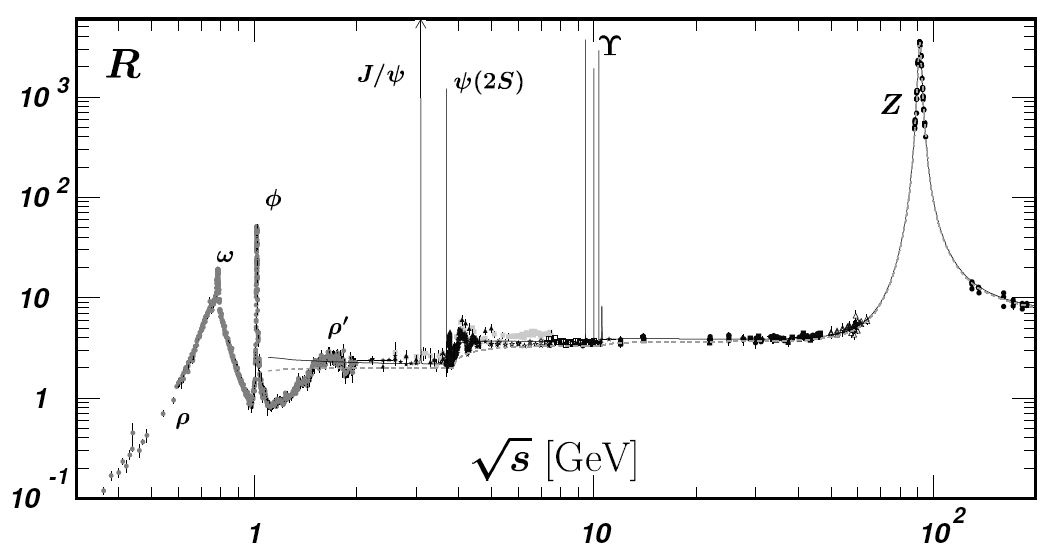
\includegraphics[width=0.8\textwidth]{Chapters/pQCD/repem.png}
% \caption{R ratio of electron positron cross section to hadrons and
%   leptons, as a function of centre-of-mass energies.}
% \label{fig:repem}
%\end{center}
%\end{figure}
%
%We see from the plot that $R$ increases with centre-of-mass energy. % in steps that are delimited by
%% approximately the centre-of-mass energy needed to produce a new quark
%% flavour.
%This behaviour is problematic, since dimensional analysis
%tells us that $R$ should be independent of the energy scale, hence
%constant when increasing the centre-of-mass energy.

% This behaviour is regularised with the formalism of renormalisation. 

% In quantum field theories, % In order to avoid discussion of renormalisation theory, I'll assume
% that $R$, which in principle should not depend of any energy scale $Q^{2}$,
% can become non-dimensional using the tools of dimensional regularisation,
% so that $R$ is now a function of the ratio $Q^{2}/\mu^{2}$.

%With
%$\alpha_S$ being a function of $\mu$ we have for $R$:
%\begin{equation}
%R \equiv R\left(\frac{Q^{2}}{\mu^{2}},\alpha_{S}(\mu)\right),
%\end{equation}
%but at a given (constant) coupling $\alpha_S^{r}$ (the one entering
%the Lagrangian), $R$ does not depend strictly on $\mu$, and can be
%expressed as $R(Q^{2}/\mu,\alpha_{S})$ such that:
%\begin{equation}
%\mu^{2}\,\frac{d}{d\mu^{2}}R\left(\frac{Q^{2}}{\mu^{2}},\alpha_{S}\right)
%\,\equiv\, \left( \mu^{2}\frac{\partial}{\partial\mu^{2}} + \mu^{2}\frac{\partial\alpha_{s}}{\partial\mu^{2}}\frac{\partial}{\partial\alpha_{S}}  \right)\,R = 0.
%\end{equation}

This partial differential equation can be simplified introducing
the following:
\begin{equation}
\tau = \textrm{ln}\left( \frac{Q^{2}}{\mu^{2}} \right),\hspace{1cm}\beta(\alpha_{S})=\mu^{2}\,\frac{\partial\alpha_{S}}{\partial\mu^{2}}
\end{equation}
We now have a \textit{renormalisation group equation} for $R$:
\begin{equation}
\left( -\frac{\partial}{\partial\tau} +
  \beta(\alpha_{S})\frac{\partial}{\partial\alpha_{S}}\right)R\:=\:0.
\end{equation}

This can be solved by defining a coupling varying with the scale, the
\emph{running coupling}:
\begin{equation}
\tau = \int_{\alpha_{S}(\mu)}^{\alpha_{S}(Q)} \frac{dx}{\beta(x)},
\end{equation}
and the way $\alpha_{S}$ varies is determined by the $\beta$
function. Anticipating that a determination of $\alpha_{S}$ with the
$\beta$ function is based on
an infinite series of ever more complicated diagrams revolving around
gluon self interactions and quark loops, let us just jump to the
result and say that $\beta$ at first order in $\alpha_{S}$ (\textit{leading
order}, or LO) is given by:
\begin{eqnarray}
\beta(\alpha_{S}) &=& -b \alpha^{2}_{S}(1 +\mathcal{O}(\alpha_{S}))\\
\vspace{0.5cm}
b &=& \frac{11 C_{A} - 2 N_{f}}{12\pi} > 0
\end{eqnarray}
where $C_A=3$ and $N_f$ the number of active flavours. The $\beta$ function values decrease as
$\alpha_{S}$ increases, and
the first order $-b$ parameter is \textit{negative}\footnote{That is,
  as long as the number of active quark flavours is $N_f < 16$.}, contrary to the two electroweak constants. For QED,
$\beta(\alpha_{QED})=\alpha_{QED}^{2}/3\pi$. It is positive, such that
the coupling increases when one resolves the charged particle with higher
and higher energies. Inversely, for quantum chromodynamics, the
coupling decreases as energy increases: this is known as \emph{asymptotic
freedom}.

Modern measurements of $\alpha_S(Q)$ will be shown in
Section~\ref{sec:alphasrunning} and we will see how well they match
with the theoretical prediction of running $\alpha_S$. 
I have decided to limit myself to the running of the coupling and
the basic structure of the Lagrangian, for the following reasons:
\begin{itemize}
\item[-] These two points are fundamental for the building of QCD, and
  make it a unique theory,
\item[-] the non-abelian term in the Lagrangian is crucial for the
  appearance of this asymptotic freedom property,
\item[-] the dynamical evolution of the coupling
  sets the basis to turn to \emph{deconfinement}.
\end{itemize}

The rest of this section will be devoted to present experimental
successes, or milestones, of QCD. 

Let us look first at a concrete quantity, that is the ratio $R$ of
cross sections for hadron production and dimuon production in
$e^{+}e^{-}$ annihilation:
\begin{equation}
R\: \eqdef \:\, \frac{\sigma(e^{+}e^{-}\to\textrm{hadrons})}{\sigma(e^{+}e^{-}\to\mu^{+}\mu^{-})}.
\end{equation}

This quantity, as plotted in Figure~\ref{fig:repem}, varies mildly and
continuously as a function of \s\ above 5~GeV, in a way that is well
reproduced by the running coupling constant (see~\cite{Agashe:2014kda}, Section
9.2.1). It also reveals striking features: resonances, and steps that are thresholds
for the production of new quarks, that I shall discuss in the next section. 

\begin{figure}[h]
\begin{center}
  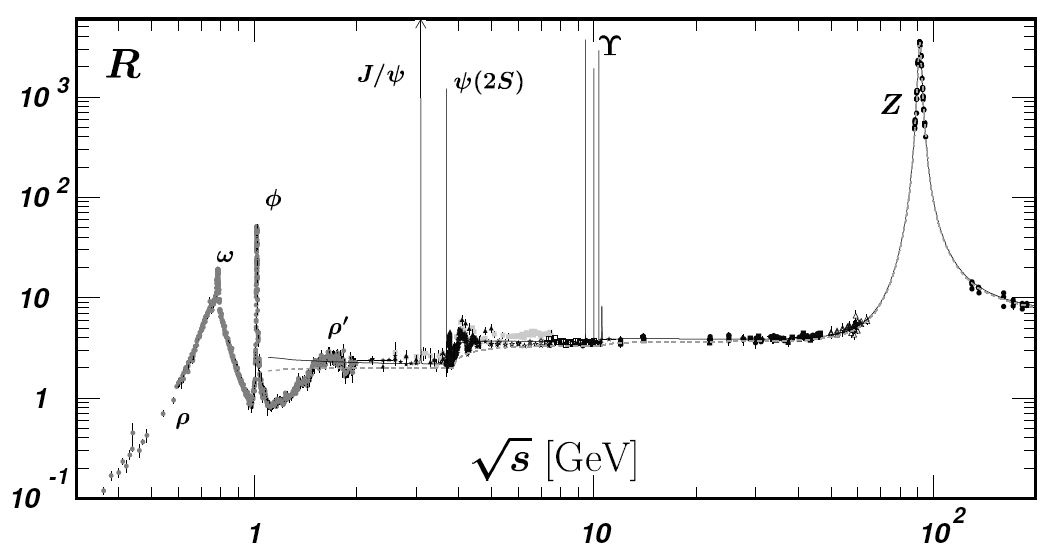
\includegraphics[width=0.8\textwidth]{Chapters/pQCD/repem.png}
 \caption{R ratio of electron positron cross section to hadrons and
   leptons, as a function of centre-of-mass energy.}
 \label{fig:repem}
\end{center}
\end{figure}

% By essence, the theory is a very
% rich one, and that's maybe where the bat hurts: if one tries to
% develop calculations outside of the perturbative regime, as in the
% case of hadronisation, one finds out fast that a non-perturbative
% treatment for QCD is hopeless. Along the same lines, perturbative QCD
% is essential for high-energy physics, in that most of the corrections
% to processes such as $t$ quark production, Higgs properties, exotic
% physics' searches, ... are all entitled to QCD calculations. One can
% compute QCD processes at leading order, or next-to-leading order, or
% maybe more. But eventually, the computation of the next order relies
% on the knowledge of what is the scale of the next-order effects, and what is going to be size of the coupling for these
% higher order processes. So it seemed to me as the non-Abelian nature
% of $\mathcal{L}$ and the
% running of $\alpha_{S}$ were all I needed for now. When I will be looking at nuclear interactions the picture
% will complexify with collectivity and finite-temperature QCD, but for now,
% I should wrap up the story, pay respects to the November Revolution,
% and salute a few famous measurements that gave to this revolutionary
% theory its full glory.

\subsection{The November Revolution}
\label{sec:november}

In Section~\ref{sec:verge}, I have argued that even though the group
theory grounds were there for QCD to be built already in the sixties, there was a lot
of skepticism regarding the existence of quarks, as well as the
number of quark flavours. At the same time, a large portion of the
theoretical physics community was working on the weak interaction
unification with QED and the renormalisability of quantum gauge field
theories. On the experimental side, strange mesons and baryons were
discovered, and their spectroscopy was well studied. The $s$ quark
mass being presumably heavier than the other two known quarks, it was
clear that hadrons carrying one or more units of strangeness would be
rather unstable. Indeed, the $\Xi$ baryons and $\Omega^{-}$ were
discovered through decay processes. But some transitions, namely the
ones with $\Delta S = 2$ remained elusive. Using the framework of
current algebra, Glashow and Bjorken put out the idea of a
\textit{fourth} quark, the charmed quark, already in 1964. The idea
was to enforce an analogy between the weak leptonic current and weak
hadronic current: if two weak lepton doublets exist, ($e$,$\nu_{e}$)
and ($\mu$,$\nu_{\mu}$), there had two be two weak doublets for quarks
as well~\cite{lai}. 

One of the doubts on the existence of quarks, before DIS experiments
came to light, was the fact that the $SU(3)_{F}$ flavour symmetry of the quark
model was a \textit{global symmetry}~\cite{luigi_gauge}. In this sense, the free fermion
fields for $SU(3)_{F}$ quarks $q_{i}(x)$ are such that:
\begin{equation}
\chi(x) = \begin{pmatrix} q_{u}(x) \\ q_{d}(x) \\ q_{s}(x) \end{pmatrix}
\hspace{1cm} \bar{\chi}(x) = \begin{pmatrix} \bar{q}_{u}(x) &
  \bar{q}_{d}(x) & \bar{q}_{s}(x) \end{pmatrix}
\end{equation}
and the Lagrangian for the three free fields is 
\begin{eqnarray}
\mathcal{L} &=& \displaystyle\sum_{i=u,d,s} \bar{q}_{i}(x)\left(
  i\gamma^{\mu}\partial_{\mu} - m\right)q_{i}(x), \\
&=& \bar{\chi}(x)\left(  i\gamma^{\mu}\partial_{\mu} - m\right)\chi(x).
\end{eqnarray}
Let us express the effect of $V$, a $U(3)$ transformation:
\begin{eqnarray*}
\chi(x) &\to& V\chi(x), \\
\bar{\chi}(x) &\to& \bar{\chi}(x)V^{\dagger}, \\
\mathcal{L} &\to& \bar{\chi}V^{\dagger} \left(
  i\gamma^{\mu}\partial_{\mu} - m \right) V\chi(x) = \mathcal{L}.
\end{eqnarray*}
Given that $U(3) = SU(3) \times U(1)$, such transformations are
unitary 3$\times$3 matrices, with unit determinant. This is the
$SU(3)$ generalised isotopic spin
symmetry of Gell-Mann's Eightfold Way~\cite{eightfoldway}, only
if the quark masses were equal! Entering quark masses would strongly hurt the symmetry to the point where it is
explicitly broken, and as Gell-Mann puts it in~\cite{eightfoldway}, 
\begin{quote}
\textsf{In the limit of unitary symmetry and with the mass of these vector
mesons "turned off'', we have a completely gauge-invariant and minimal
theory, just like electromagnetism. When the mass is turned on, the
gauge invariance is reduced (the gauge function may no longer be
space-time-dependent) but the conservation of unitary spin remains
exact. [...] there are also the many symmetry rules associated with
the unitary spin. All of these are broken, though, by whatever
destroys the unitary symmetry, and it is a delicate matter to find
ways in which these effects of a broken symmetry can be explored experimentally.}
\end{quote}

From there, we can easily imagine what harm it would do to include a
fourth, heavier quark in any such model. In a quite different attempt
to understand flavour-changing currents, Glashow, Iliopoulos and
Maiani~\cite{GIM_mechanism}, suggested in 1970 a mechanism which explains how
the flavour changing process $K^{0}\to \mu\mu$ is naturally rare. A
simple picture of the GIM mechanism is presented in the
Figure~\ref{fig:GIM}. They postulate the existence of a fourth quark,
$c$, that would have the charge +2/3 as the $u$ quark.

\begin{figure}
\begin{center}
  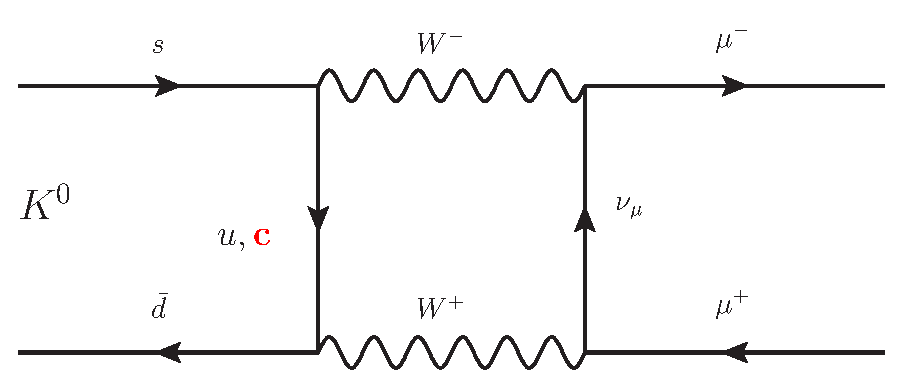
\includegraphics[width=0.6\textwidth]{Chapters/pQCD/GIM.pdf}
 \caption{The GIM mechanism in $K^{0}\to \mu\mu$ decay. Note the
   appearance of a charm quark contribution inside the box diagram.}
 \label{fig:GIM}
\end{center}
\end{figure}


For the next four years the charm quark existence was largely
overlooked. During the summer of 1974, Ting and his research team
started accumulating proton-proton data from the AGS at Brookhaven, hinting at the production of a new, very narrow
resonance of mass $\sim$ 3.1~GeV/$c^2$. Because of the very narrow aspect
the resonance had, it did not go into immediate publication. On
November 10, 1974, the team led by Richter who was operating the SPEAR
electron-positron collider at SLAC discovered that at beam energies
around E$_{b} \sim$ 
1.55 GeV, the counters went berserk. On November 11, 1974, both
collaborations at Stanford and Brookhaven announced their discoveries
of the \Jpsi~particle, which was quickly interpreted as a resonant
$c\bar{c}$ state, that is, a bound state of a charm quark and an anti-charm quark.

\begin{figure}[h]
\begin{center}
  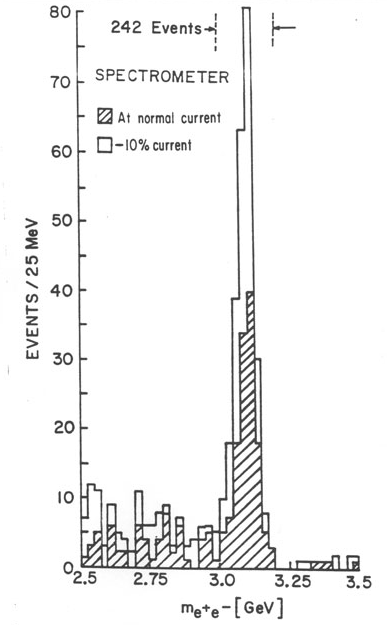
\includegraphics[width=0.25\textwidth]{Chapters/pQCD/psi_bnl.png}
  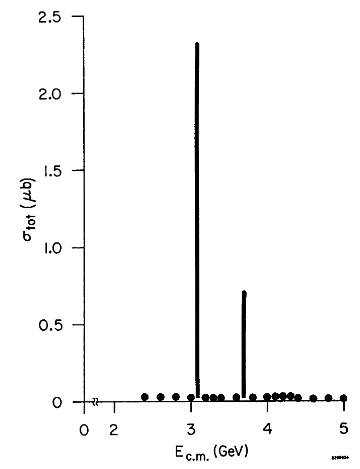
\includegraphics[width=0.3\textwidth]{Chapters/pQCD/psi_slac.png}
 \caption{First charmonium data. Left: statistics accumulated at
   BNL~\cite{psi_bnl}. Right: $e^{+}e^{-}$ events from SPEAR, showing a second
   resonance, the $\psi'$~\cite{psi_slac}.}
 \label{fig:psi}
\end{center}
\end{figure}

Two weeks later, in an energy scan for new particles in the charmonium
spectrum, excitement
struck again as the team at SPEAR discovers a second narrow resonance,
as can be seen in Figure~\ref{fig:psi}. One can see on the plot to the
right, events stacking at 3.1~GeV/$c^2$ and at 3.7~GeV/$c^2$, indicating the
presence of the $\psi'$. Only two years later, both Richter (SLAC) and
Ting (MIT) received the Nobel Prize in Physics ``for their pioneering
work in the discovery of a heavy elementary particle of a new kind''.

Shortly thereafter, the $\tau$ lepton was discovered at the SPEAR
facility~\cite{Agashe:2014kda}. This new lepton, discovered indirectly
through its weak
decay in $e^{+}e^{-}\to\tau^{+}\tau^{-}\to\mu^{\pm}e^{\mp}+2\nu$ came
first as an anomaly, before DESY confirmed the
signal. After establishing the quantum numbers of the newly-discovered
particle, it became clear that a new family of leptons was
released. With this discovery, the community soon concluded that two
additional quarks, $b$ and $t$ for bottom and top (or beauty and
truth) were to be expected. And indeed, in 1977, after seeing a hint
of a bump at $m \sim 9.6$~\unitMass\ prior to a significant upgrade, the
E288 collaboration (Lederman et al.) published their observation of
a new resonant structure in the di-lepton decay
channel~\cite{lederman}, which turned out to be the \PgU\ family, of particular interest for this thesis. 

\begin{figure}[h]
\begin{center}
  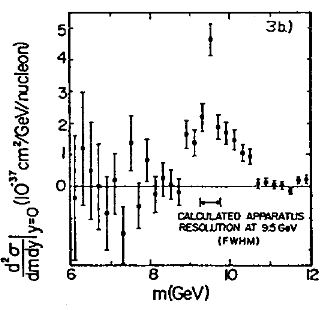
\includegraphics[width=0.5\textwidth]{Chapters/pQCD/first_ups.png}
 \caption{First bottomonium data, 1977. Dimuon events from proton-nucleus collisions
 at $E_{p}$ = 400 \GeV\ with the E288 experiment at Fermilab~\cite{lederman}.}
 \label{fig:upsi}
\end{center}
\end{figure}

\subsection{The discovery of the gluon}

% On the aftermath of the November revolution, there remained one grey
% area in the strong interactions. 
It is now clear that quarks exist
confined in the nucleons, and are probed only when increasing the
scattering energy enough so that the Compton wavelength of the
exchanged photon (in the case of DIS) is much smaller than the size of
the nucleon wavefunction. And doing so, we have seen in Equation~\ref{eqhalftheproton} that the
momentum fraction carried by the quarks was only
approximately half of the total available nucleon momentum. So it
seems clear that the colour field holding quarks in place is naturally
giving rise to other objects contributing to the nucleon integrity.


A recent account by Ellis~\cite{gluon_ellis} makes a very interesting
report of the events that led to think of strong interactions in term
a non-abelian $SU(3)$ theory. The first experimental signature
involving gluons in the final state was to be formulated in a 1976 paper by
Gaillard, Ellis and Ross, where they compute the gluon
bremsstrahlung\footnote{From the German word for ``deceleration radiation''.}
process in QCD~\cite{qqg} at $e^{+}e^{-}$ facilities, stating that it
should give rise to $q\bar{q}g$ final states. This final state is
observed experimentally in the form of three distinct clusters of
particles, further called~\textit{jets}.

\begin{figure}[t]
\begin{center}
  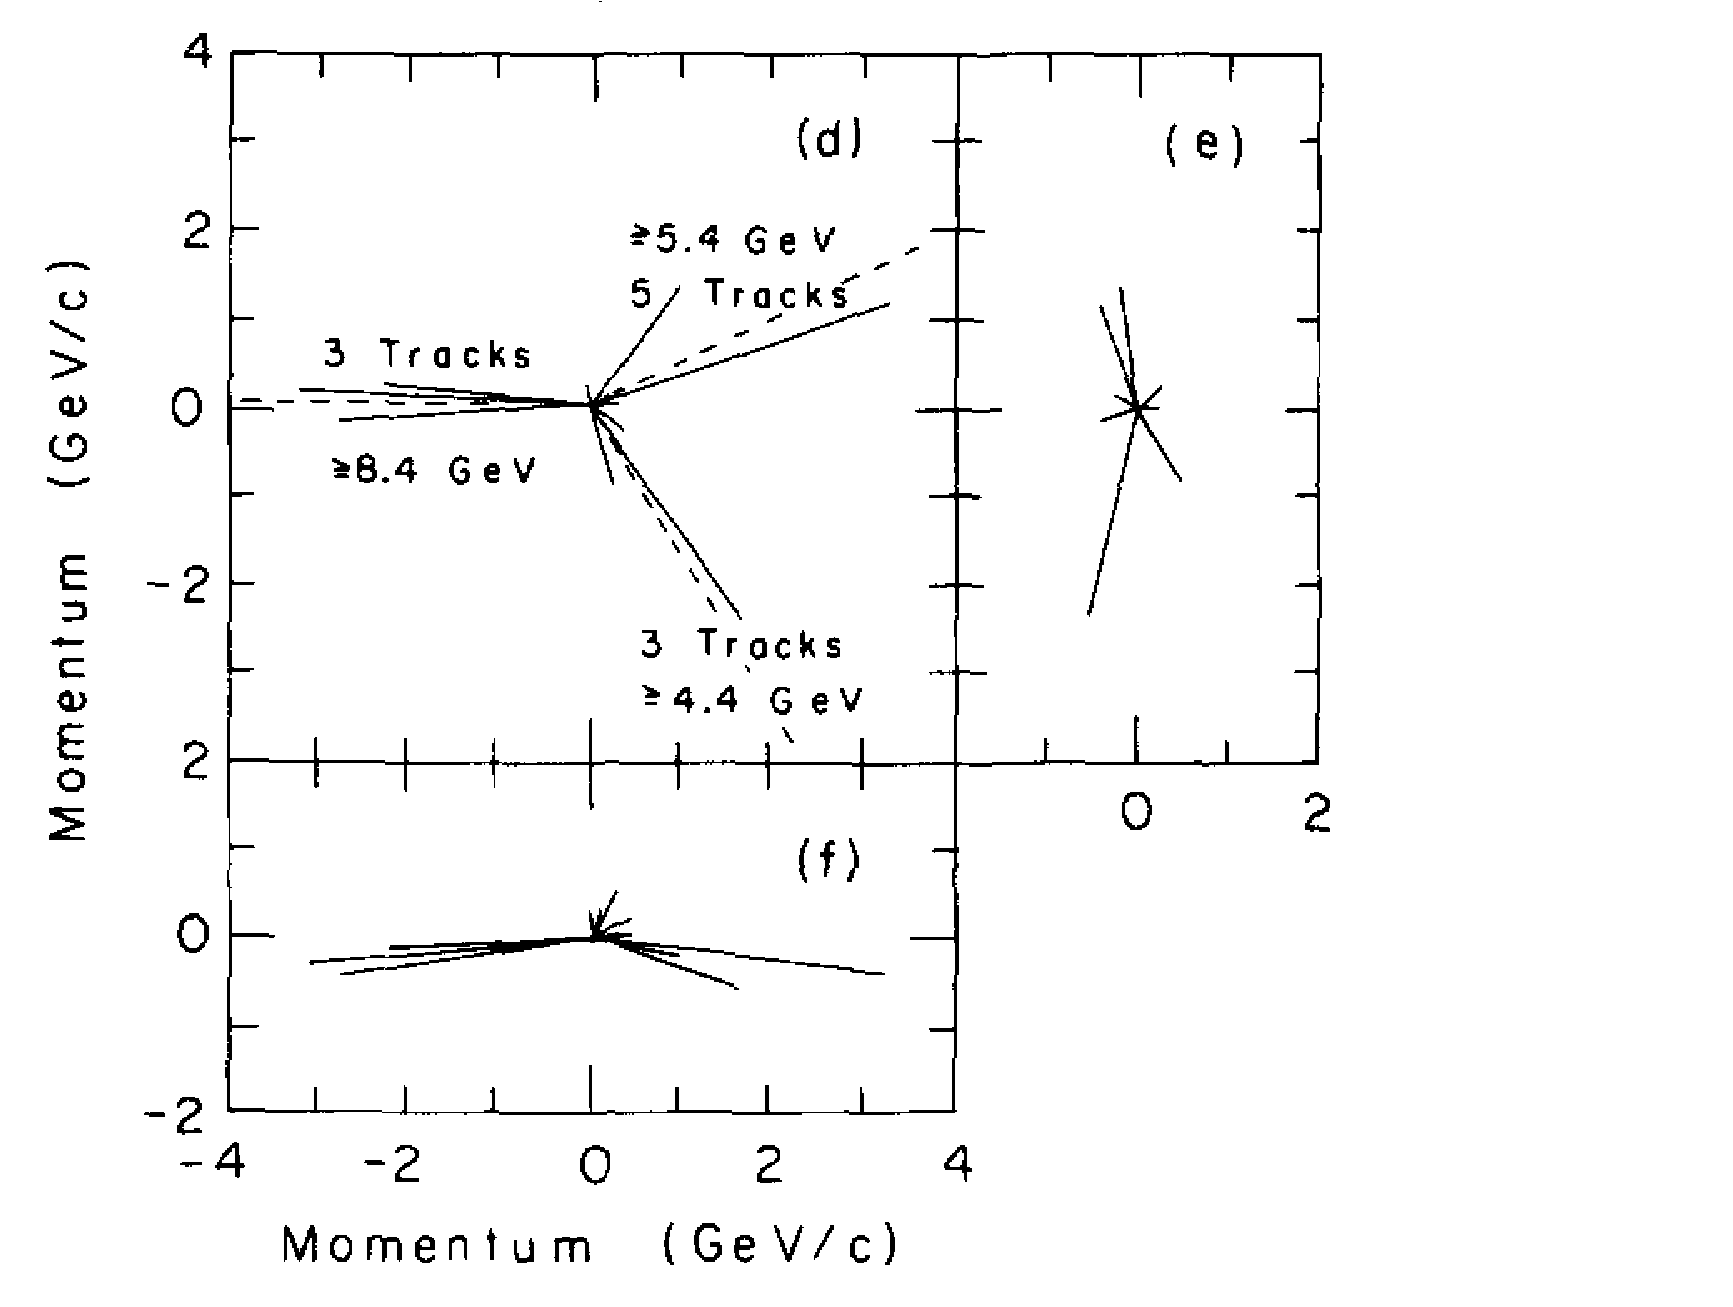
\includegraphics[width=0.7\textwidth]{Chapters/pQCD/qqg.png}
 \caption{A three-jet $q\bar{q}g$ event, from the TASSO collaboration \cite{wiik}.}
 \label{fig:gluonJet}
\end{center}
\end{figure}


Circumstantial evidence that gluons did exist was already
available. For example, charmonium and bottomonium decays to
three gluons, were computed to be the dominant decay mode for these
new objects. The discovery of the gluon radiation in 3-jet
events, and hence of its survival
to the long-distance process of hadronisation was announced jointly by
all four PETRA experiments at a Fermilab Lepton-Photon Symposium in
August 1979~\cite{tasso_g}. Figure~\ref{fig:gluonJet} shows one of the first such
$q\bar{q}g$ events recorded by the TASSO collaboration, where the three jets are easily seen in
the transverse plane (main panel).

This evidence for gluon bremsstrahlung is actually the basis for the
crucial QCD test described hereafter. 

\subsection{Testing QCD at \texorpdfstring{$e^{+}e^{-}$}{e+e-}, DIS
  and hadron colliders}
I will go briefly through several selected results from QCD analyses of
collider data from the eighties and nineties, which confirmed with
great accuracy many features of
\textit{perturbative}
% \footnote{A -- Non-perturbative effects require much
%   more computational power because of the many divergences. B --
%   Colour confinement should find a dynamical explanation, which is yet
% unknown.} 
QCD dynamics, as imposed by Equation~\ref{eq:qcdlagrangian}. 

\subsubsection{The non-Abelian nature of QCD}

The QCD Lagrangian discussed in Section~\ref{sec:lagrangian}, contains Feynman
diagrams with three-gluon and
four-gluons vertices. This is a specificity of the non-Abelian nature
of $SU(3)$, which has many consequences for the amplitude of various
processes. One example: 4-jet events in $e^{+}e^{-}$  collisions are
produced with tree-level QCD diagrams of Figure~\ref{fig:gluons}. Such
events will produce four clustered energy deposits (known as
\textit{jets}) in the final state, from which one can for example make
an event shape analysis.
\begin{figure}
\begin{center}
    \begin{subfigure}{0.244\textwidth}
      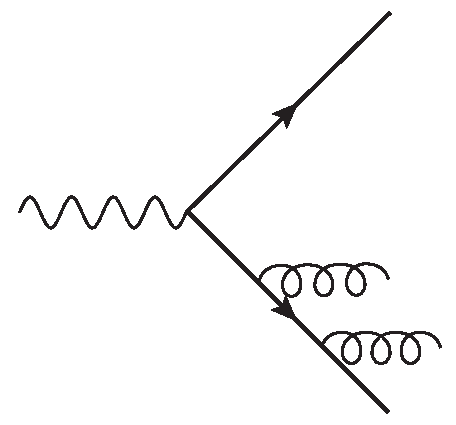
\includegraphics[width=\textwidth]{Chapters/pQCD/gluon1.pdf}\caption{}\end{subfigure}
    \begin{subfigure}{0.244\textwidth}
      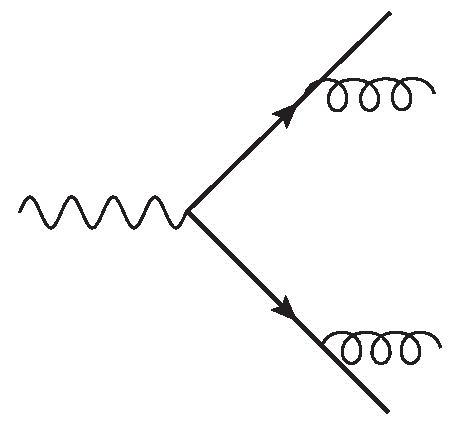
\includegraphics[width=\textwidth]{Chapters/pQCD/gluon2.pdf}\caption{}\end{subfigure}
    \begin{subfigure}{0.244\textwidth}
      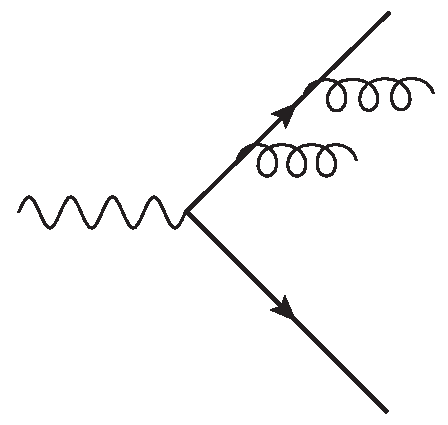
\includegraphics[width=\textwidth]{Chapters/pQCD/gluon3.pdf}\caption{}\end{subfigure}
\hfill ~\\
    \begin{subfigure}{0.244\textwidth}
      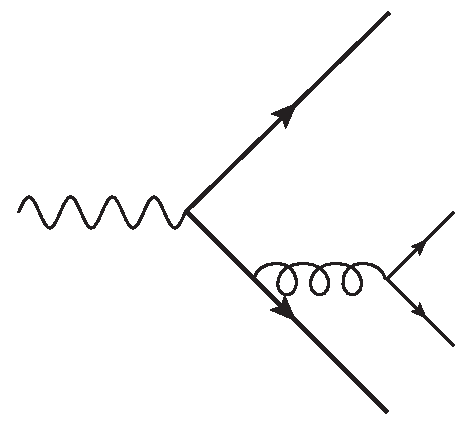
\includegraphics[width=\textwidth]{Chapters/pQCD/gluon5.pdf}\caption{}\end{subfigure}
    \begin{subfigure}{0.244\textwidth}
      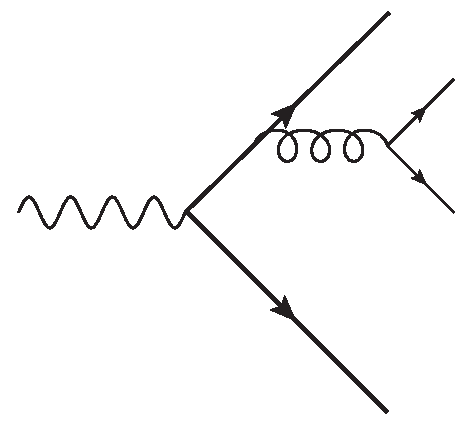
\includegraphics[width=\textwidth]{Chapters/pQCD/gluon6.pdf}\caption{}\end{subfigure}
    \begin{subfigure}{0.244\textwidth}
      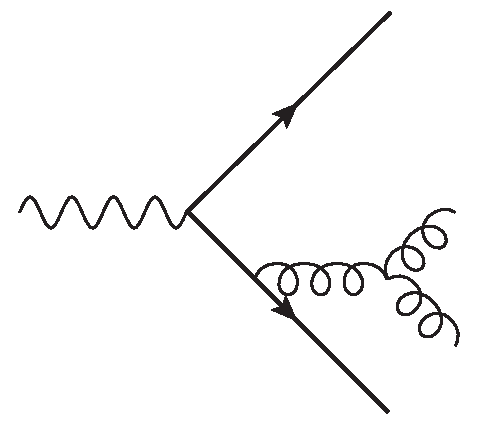
\includegraphics[width=\textwidth]{Chapters/pQCD/gluon7.pdf}\caption{}\end{subfigure}
    \begin{subfigure}{0.244\textwidth}
      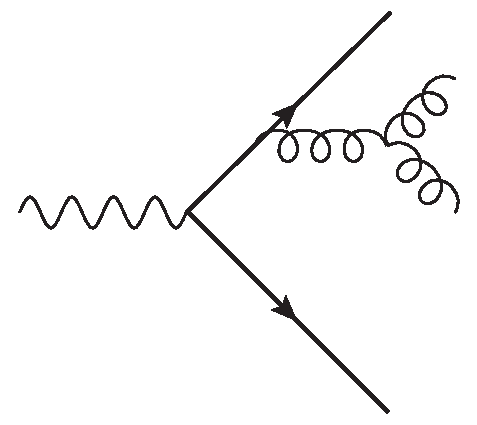
\includegraphics[width=\textwidth]{Chapters/pQCD/gluon8.pdf}\caption{}\end{subfigure}
    \caption{Tree-level Feynman diagrams for four jet events in electron
      positron collisions.}
    \label{fig:gluons}
\end{center}
\end{figure}


Take the four jet momenta ($p_1$, $p_2$, $p_{3}$, $p_4$) such that
they are energy ordered, $E_1 > E_2 > E_3 > E_4$. Most
likely the first two most energetic jets will come from the
quark lines, and one can define a plane $\mathcal{P}_{1,2}$. The question
is to know the angle between the plane $\mathcal{P}_{1,2}$ and the
plane delimited by the two sub-leading jets $p_3$ and $p_4$,
$\mathcal{P}_{3,4}$. First let me point out that double-bremsstrahlung diagrams (a), (b) and
(c) do not contribute very much to the correlation angle between
$\mathcal{P}_{1,2}$ and $\mathcal{P}_{3,4}$. 

Next, if gluon
radiation was like photon radiation in electromagnetism, i.e. Abelian,
then there would be no $g\to gg$ terms. There would then only be the
four-quark diagrams (d), (e). These would contribute as a
strong anticorrelation: Indeed, one can conclude from the gluon
polarisation that radiated gluons tend to be polarised in the plane
of the primary jets, and will split in two quarks of perpendicular
direction with respect to the $g$ polarisation. So diagrams (d), (e)
would give a wide angle between $\mathcal{P}_{1,2}$ and
$\mathcal{P}_{3,4}$. 

% Note that the colour factor for $g\to q\bar{q}$ is $C_{F}$ = 4/3 in QCD.

\begin{figure}
\begin{center}
  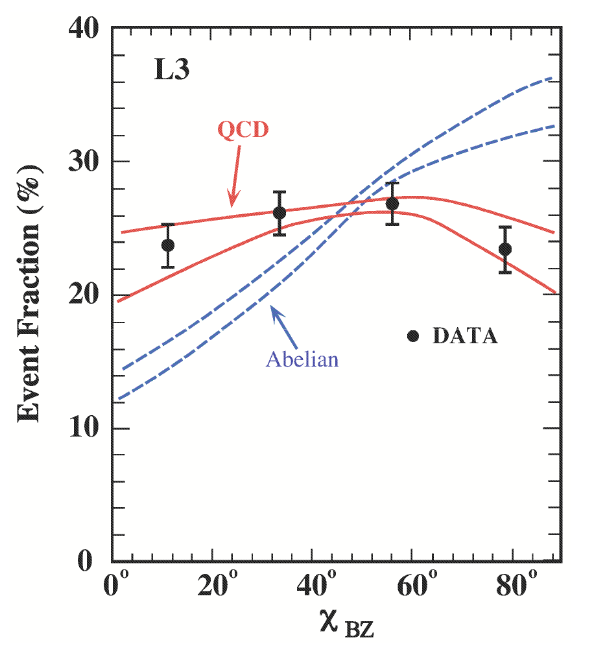
\includegraphics[width=0.5\textwidth]{Chapters/pQCD/xbz.png}
 \caption{The Bengtsson-Zerwas angle $\chi_{BZ}$ in four-jet events recorded by
   the L3 collaboration~\cite{xbz_l3}.}
 \label{fig:xbz}
\end{center}
\end{figure}


Finally, because of the non-Abelian nature of QCD, one has to consider
diagrams (f) and (g). It turns out that $g \to gg$ is dominant in QCD, by
virtue of the colour factor $N_{c}$ = 3, as well as the soft gluon
enhancement. Still using the
polarisation properties of gluon emission, the first gluon is radiated
along the plane $\mathcal{P}_{1,2}$, splitting in two gluons this time
mostly parallel to the polarisation. This correlation is weak but the
process is very abundant, resulting in a clear flattening of the
angular distribution in Figure~\ref{fig:xbz}. 

The angle $\chi_{BZ}$
used herein is called the Bengtsson-Zerwas angle~\cite{xbz}, defined by the
plane between the two leading jets and the two subleading jets. The
data from L3 collaboration is compared to a full-fledged QCD
simulation as well as to a straw-person model where
only Abelian terms are allowed. The Abelian theory curve is indeed peaking at
$\chi_{BZ} \sim \pi/2$, and does not match with the experimental data, indicating that the data does conform to
a non-Abelian theory.

Such four-jet analyses can be combined with other event shape analysis
and 3-jet events to yield a precise evaluation of QCD colour
factors. Figure~\ref{fig:combiLEP} presents a famous combination of results from LEP experiments (OPAL,
ALEPH, DELPHI) that shed light on the true value of QCD colour factors,
further confirming the $SU(3)$ group as its underlying theoretical structure.

\begin{figure}
\begin{center}
  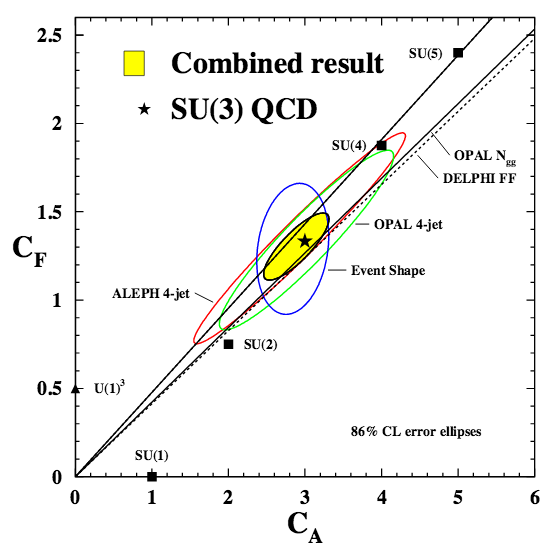
\includegraphics[width=0.5\textwidth]{Chapters/pQCD/combiLEP.png}
 \caption{The LEP-combined plot of $C_{A}$ and $C_{F}$. The yellow
   ellipsoid area is the combined uncertainty of the various jet and
   event shape measurements. Taken from~\cite{webber2}.}
 \label{fig:combiLEP}
\end{center}
\end{figure}

\subsubsection{Precision measurements of QCD effects}
Since the first attempt at measuring precisely $\alpha_{S}$ at the
time of PETRA and PEP colliders, many different processes from
$e^{+}e^{-}$ annihilation as well as lepton-hadron scattering gave
estimates of $\alpha_{S}$ with increasing precision. The total
hadronic cross section ratio $R$, the three-jet rate, event
shape observables, all yield experimental results on $\alpha_{S}$. It
may be worth noting that the JADE collaboration did find out a clear
experimental confirmation of the running of $\alpha_{S}$ in the rate
of three-jet events, already before the coupling constant value was
precise; back then, the data was compared to analytic QCD computations
at next-to-leading order in perturbation theory, including various
hadronisation models which performed relatively well, giving
$\alpha_{S}$ a mere 10\% precision~\cite{Bethke}.

The QCD programme at LEP, among other key results proving the
non-Abelian nature of QCD (cf. previous subsection) reduced
considerably these uncertainties, with $\mathcal{O}(\alpha_{S}^{3})$
precision observables: at the end of the LEP2 operation phase, the
world average was $\alpha_{S}(M_{Z})$ = 0.1184 $\pm$ 0.0031
(NNLO)~\cite{Kogler}.

Along came HERA (\textit{Hadron Elektron Ring Anlage}), at DESY in
Hamburg, with its two operation eras fully dedicated to lepton-hadron
scattering. Operating at $E_{e} = 27.5$ \GeV, and $E_{p} = (820, 920)$
\GeV, the HERA experiments (H1, ZEUS, HERMES) have accumulated, up to
2007, DIS data in an impressive phase space interval:
\begin{eqnarray*}
0.045 \: \textrm{GeV}^{2} <& Q^{2} &< 5.10^{5} \: \textrm{GeV}^{2}, \\
6. 10^{-7} <& x_{B} &< 0.65
\end{eqnarray*}

Capabilities of HERA experiments are very large: thanks to the
precise data accumulated in charged-current and neutral-current modes,
the QCD contributions to all processes, and the various parton PDFs can be computed
simultaneously. For example, inclusive jet cross section is measured
to the level of precision that one can see from ZEUS data in
Figure~\ref{fig:zeus} and compared to NLO QCD perturbation theory predictions. From that one
can extract for example $\alpha_{S}$, or measure the charm or bottom
quark mass with precision~\cite{H1Charm}. Figure~\ref{fig:zeus} (right) shows a
comparison of $\alpha_{S}$ from inclusive jets to NLO QCD
calculations, where the main sources of theory uncertainty come from
the various assumptions on either the perturbative part (DGLAP
evolution equations~\cite{Dokshitzer:1991wu}) or the PDF. 

\begin{figure}[htb]
\begin{center}
  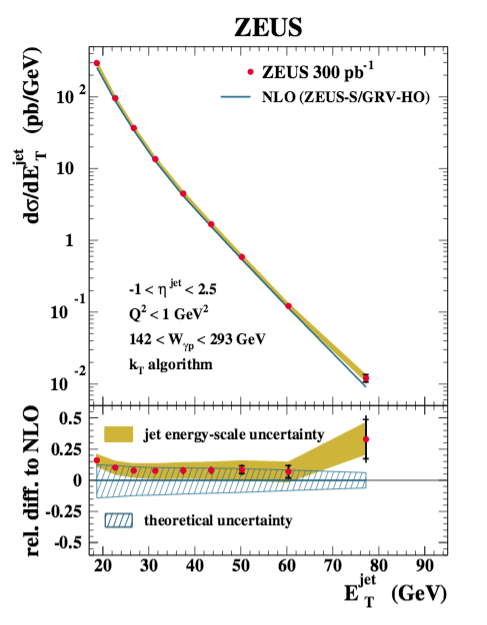
\includegraphics[width=0.35\textwidth]{Chapters/pQCD/zeus_jetCS.png}
  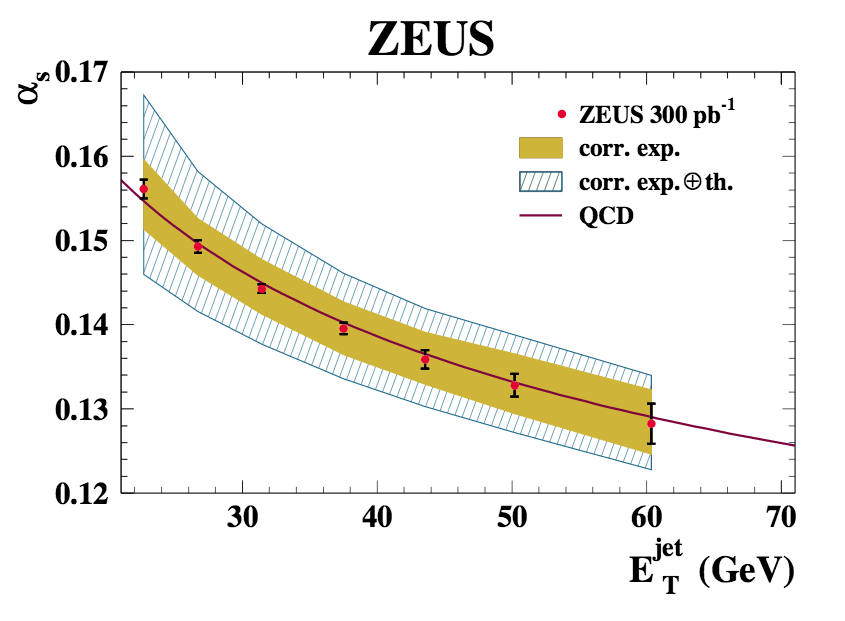
\includegraphics[width=0.63\textwidth]{Chapters/pQCD/alpha_s_zeus.png}
 \caption{Inclusive jet productions from the ZEUS collaboration. Left:
   the p$_{T}$ differential cross section. Right: $\alpha_{S}$. In both
   plots comparisons to dedicated NLO QCD calculations are shown. Taken from~\cite{Paul}.}
 \label{fig:zeus}
\end{center}
\end{figure}

This is only one small account of the various successes of QCD. In 2015, HERA experiments released a seminal paper
updating their long-collected parton PDF data~\cite{HERA_END}. One of the most
striking figures is reproduced as
Figure~\ref{fig:DIS_HERA}, where the quark and gluon PDFs are
reproduced at NNLO at a very close level of precision with fits
to data. This genuine piece of information will provide important
tuning to the study of hadron-hadron processes at LHC experiments. Indeed, almost all
processes (especially the most challenging ones, e.g. searches for Higgs
couplings to quarks) rely heavily on parametrising the momentum fraction carried by
gluons and quarks in the proton. For heavy quarkonia this also plays a
role, as gluon fusion is the dominant process at
LHC energies.

\begin{figure}[htb]
\begin{center}
  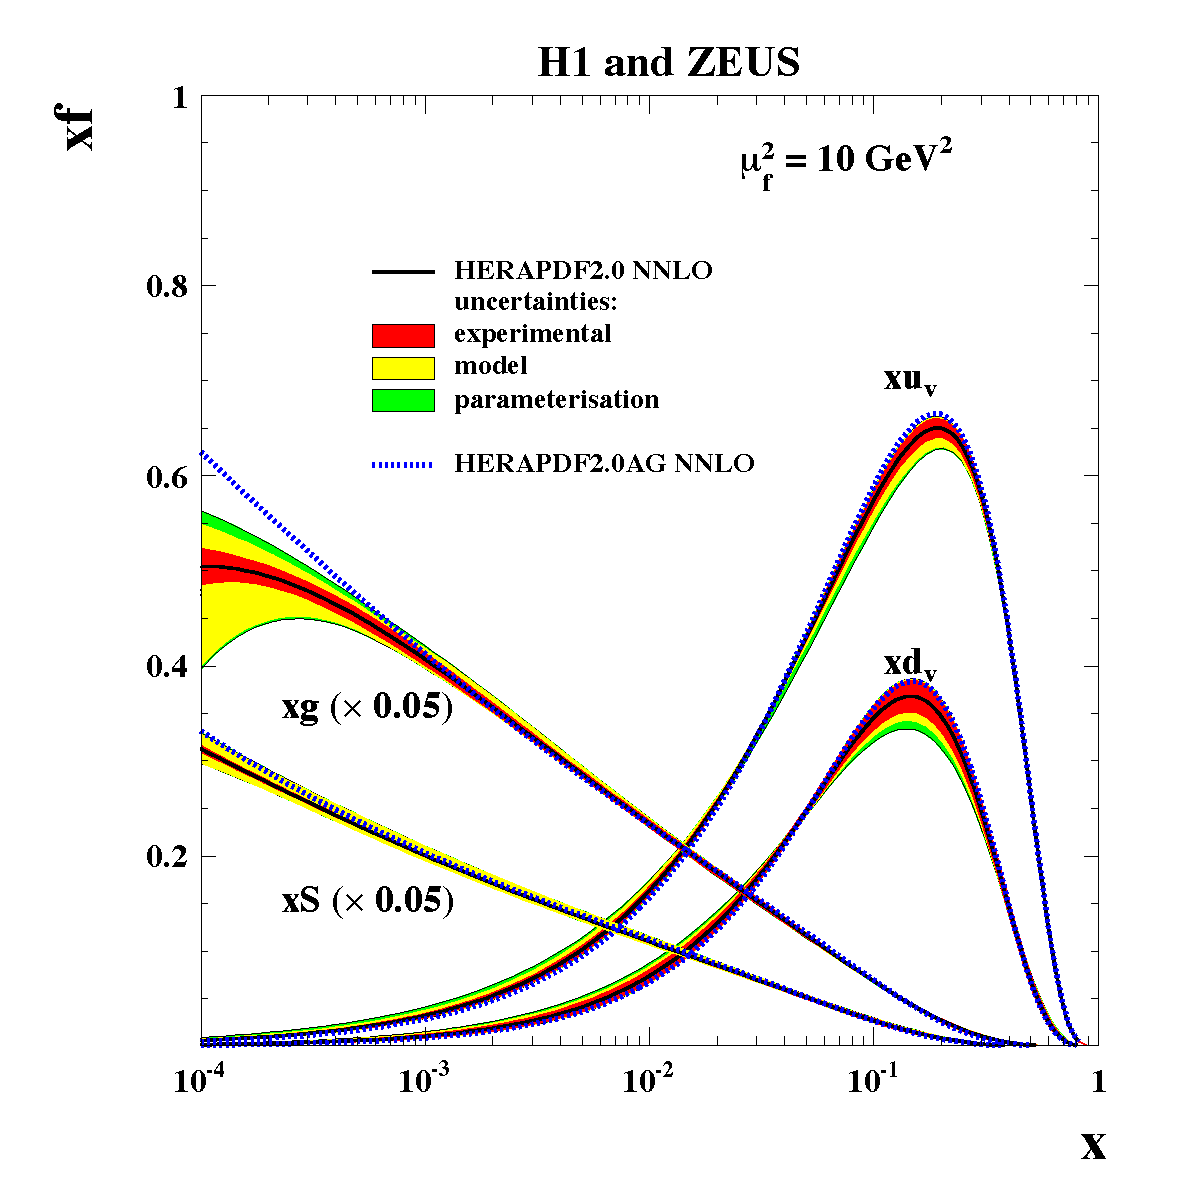
\includegraphics[width=0.65\textwidth]{Chapters/pQCD/DIS_HERA.pdf}
 \caption{Parton distribution functions $xu_v$, $xd_v$, $xS =
   2x(\bar{U}+\bar{D})$ and $xg$ of HERAPDF2.0 NNLO at $\mu_{\rm f}$ =
   10 GeV$^{2}$~\cite{HERA_END}. Gluon and sea distributions are scaled down by a
   factor of 20.}
 \label{fig:DIS_HERA}
\end{center}
\end{figure}

% \vfill\newpage

\subsubsection{Modern running coupling constant measurements}
\label{sec:alphasrunning}

Finally, the best illustration of QCD success is the comparison of its
predicted running of $\alpha_S$ with experimental measurements related
to this quantity, at various orders of perturbation theory. This is
presented in Figure~\ref{fig:alphasrunning},
from~\cite{Agashe:2014kda}. Nowadays, the running of $\alpha_S$ is
well understood, and is of prime importance for a large majority of
Standard Model physics analyses. Indeed, almost every rare physics
process studied at the LHC is usually extracted from the sum of several
templates of signals whose cross section is known to
several orders of the strong coupling constant. The precise knowledge
of QCD is crucial also in the modelling of~\textit{hadronisation},
which is the process by which final state particles radiate softer
particles and form detectable jets.

\begin{figure}[h]
\begin{center}
  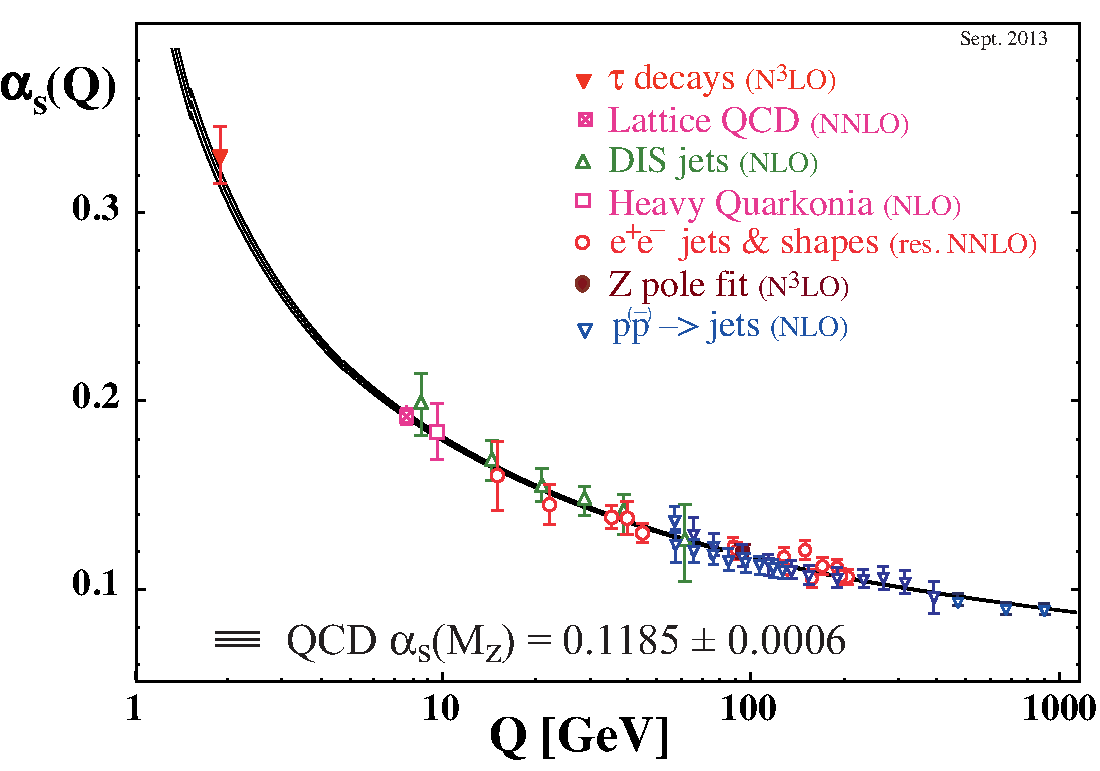
\includegraphics[width=0.8\textwidth]{Chapters/pQCD/asq-2013.pdf}
 \caption{The running of the coupling constant of QCD~\cite{Agashe:2014kda}.}
 \label{fig:alphasrunning}
\end{center}
\end{figure}

 % The running of the coupling constant, which I have
% tried to detail down to the renormalisation group equation, gives a dynamical
% reason for quark confinement, and that is a unique aspect of QCD.
% The fact that
% there are three colour charges, and that force carriers may interact
% together, is a specificity of QCD. Of course
% all non-Abelian theories have a self-coupling for gauge
% fields, but in the particular case of QCD, the gauge fields are
% massless and this interaction plays an enormous role, starting from
% relatively low energies. 

\vspace{0.5em}
\begin{center}
  \fbox{
    \parbox{0.9\textwidth}
    {\textsf {In this section I have presented how the quantum theory for
        quarks and gluons came to be constructed, and to show some of its
        basic properties. \\ One of the key open questions of QCD is colour
        confinement. What actually drives the colour charges to equilibrate
        together and cancel themselves in the final state? What are
        the thermodynamical properties of a many-body system of colour
        degrees of freedom ?  % happens when one simulates such a system of 
        % massive and massless objects exchanging the colour quantum numbers,
        % one turns up the temperature and increases the pressure on the system?
        % What happens when the charges are getting closer and closer to each
        % other
        ? What experimental
        possibilities are available today to assess these questions? That is
        what the next section is about.
      }}} 
\end{center}

\clearpage

\section{From confinement to deconfinement}

\subsection{Phase transition at finite temperature}

Contemporary to the quark model is the discovery of microwave
background. The idea had peered through that the universe \textit{cooled down} to the T$\sim 3K$ measured in 1965,
providing evidence for a hot primordial universe. At the same time,
people studying nuclear interaction in high-energy collisions were
trying to predict the particle yields in a self-consistent
way. Hagedorn's hypothesis~\cite{Hagedorn} is worth mentioning at this point, since it
connects directly with the deconfinement sought in current day
high-energy nuclear interactions. His statistical bootstrap model
suggests that the density of hadronic states as a function of their
mass, $\rho(m)$, must be
asymptotically equivalent to the particle yields, $\sigma(E)$:

\begin{equation}
log(\rho(m)) = log(\sigma(E))
\end{equation}

Indeed, Hagedorn went on to conjecture a set of equations for
$\rho(m)$ and $\sigma(E)$ that would satisfy this criterion. In the
asymptotic limit, it translates into a density of available states which
increases exponentially with the mass:
\begin{equation}
\rho(m) \approx e^{\frac{m}{T_{H}}}
\end{equation}

and $T_{H}$ is called the Hagedorn temperature, of a value around 170 MeV. At
this temperature, the partition function becomes singular. It was
deduced that in a hot Big Bang model, the universe did produce a
wealth of unstable particles which eventually cooled down, but with
Hagedorn's temperature one could foresee that about 10 microseconds
after the Big Bang, the temperature of the universe was around 170
MeV.

In 1975, Cabibbo and Parisi~\cite{cabipari} suggested that the exponential decrease in
spectrum ($\sigma(E)$) is in fact connected to the existence of a
deconfined phase for quarks, transition that was thought to
occur at $T_{H} \sim$ 170 MeV.

So the immediate question comes along: Can we recreate this in laboratory
conditions, using ultrarelativistic nuclear beams? It should be
possible to ramp up the energy of the beams and collide enough
hadronic matter in a small volume as to increase the density and
eventually probe the existence (or absence) of this deconfinement
transition.

\begin{figure}[h]
\begin{center}
  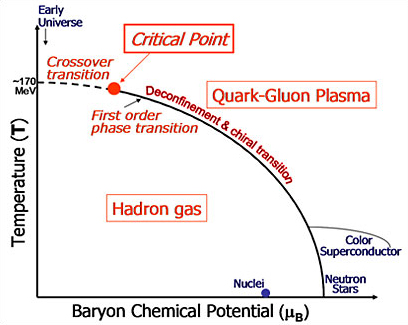
\includegraphics[width=0.8\textwidth]{Chapters/pQCD/phase.jpg}
 \caption{A schematic approach to the QCD phase transition.}
 \label{fig:transition}
\end{center}
\end{figure}

Figure~\ref{fig:transition} shows how the temperature and the baryon
chemical potential $\mu_{B}$ are related in the current picture of the phase
diagram. 

The study of the QCD phase transition with calculations on the lattice
helped drawing the thermal properties of a strongly interacting set of
objects (fermions and/or bosons) enduring increasing temperature and
pressure. For pure gluonic matter for example, the equation of state
from~\cite{lattice_g} shows a rapid approach toward an ideal gas
behaviour.
Increasing computational power helped increasing the complexity of
lattice simulations. Eventually, the energy-density/temperature
profile of models including two or three degenerate flavours of quarks
was computed and compared to what experiments were able to
perform. Figure~\ref{fig:tc_lattice} from~\cite{Karsch:2001cy} shows
such a comparison, where we 
see that the transition temperature is at T$_{c} = (173 \pm 15)$ MeV
for two quark flavours, and is accessible at the Super Proton
Synchroton (SPS) at CERN as well as at the
Relativistic Heavy Ion Collider (RHIC) at Brookhaven National
Laboratory (BNL).


\begin{figure}[h]
\begin{center}
  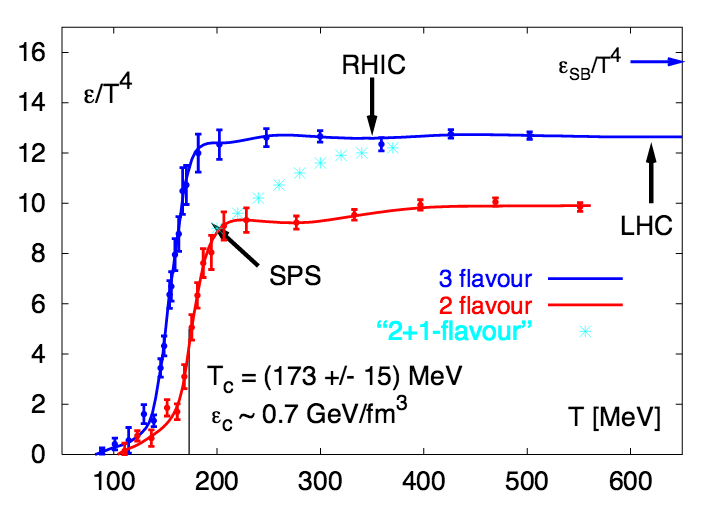
\includegraphics[width=0.8\textwidth]{Chapters/pQCD/phase_tc.png}
 \caption{Lattice calculations of the energy density as a function of
   lattice temperature, from~\cite{Karsch:2001cy}.}
 \label{fig:tc_lattice}
\end{center}
\end{figure}

There are currently two laboratories able to put the conditions
together to study the phase transition. At BNL,
RHIC collides protons, deuterons, gold nuclei, and more. For
gold-gold collisions, the energy in the centre of mass reaches
\snn\ = 200 \GeV. At CERN, fixed target experiments near the
SPS reached a \snn\ $\approx$ 17 \GeV, while
the LHC can provide lead beams to CMS, ALICE, ATLAS, and LHCb
detectors, reaching a \snn\ = 5.1~TeV in PbPb collisions\footnote{As I write this, these collisions have not yet started but correspond to the 13~TeV pp collisions that are currently ongoing.}.

If the thermal behaviour of nuclear matter under extreme pressure and
density can be studied, one can wonder what is the time evolution of
the hot medium produced. % of
% the experimental conditions
 Indeed, the deconfined phase sets
in progressively% when the strange quark mass is relatively high
% compared to the two other light quarks
\footnote{This is a \textit{crossover} instead
of a phase transition.}. In Figure~\ref{fig:timescales} the
timescales of the various processes thought to occur in
ultrarelativistic heavy ion collisions are layed out.

\begin{figure}
\begin{center}
  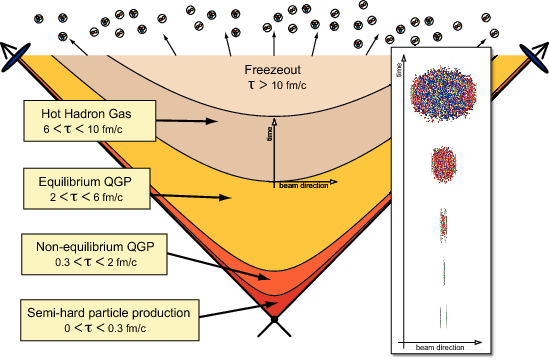
\includegraphics[width=0.75\textwidth]{Chapters/pQCD/timescales.png}
 \caption{A time frame cartoon for the thermodynamics of the QGP in
   heavy ion collisions. Both
   diagonals represent the light-cone projection of incident
   beams. The overlay on the right shows the evolution in the
   laboratory frame. From~\cite{strickland_phase}.}
 \label{fig:timescales}
\end{center}
\end{figure}


% I am getting closer to the main questions that my analysis topic is
% aiming at.
I have asserted that colliders such as LHC and RHIC should be
able to produce a deconfined phase of QCD, known as the Quark-Gluon
Plasma (QGP). Now we should try to find out what are the properties of
the 'little bang' produced in laboratory, and how can we build
strategies to probe this little bang efficiently? Finally, how can
experimental observation be related to the predicted transition?

\subsection{Measuring the properties of the quark-gluon plasma}

In DIS experiments, physicists have been able to identify and %  speculate and deduce from
% colourless 
probe the distribution of point-like objects and the force
binding them together inside the nucleons. In a way, experimental
heavy ion collisions can follow the same strategy. If we were able to
use as a probe, one object not interacting strongly with nuclear matter,
then it should be possible to use the alteration of
the probe passing through to extract physics on the created medium. I am intentionally using loose terms.
For now, let us set some rules:
\begin{itemize}
\item[1] I do not know beforehand what to expect from colliding nuclei, from
  textbook, that are mostly dealing with zero temperature particle physics;%  to Kennedy Jr.'s plane being absorbed into a
  % black hole, simply because the phenomenology detailed above could be wrong
  
\item[2] I anticipate that some probes may be
  very altered, some less. We would be interested in the spectrum of each
 type of probe, passing through whatever was created, as much as 
  in their normalisation: their total yield can carry information about the phase they traversed;
\item[3] I can however anticipate that if my experimental settings
  reach the deconfinement transition, effects on some probes would be very clear: I need a baseline for whatever would happen before
  the transition. This is crucial if my transition is continuous, from
  vacuum QCD to above the critical density.
\item[4] Finally, I need to get an experimental handle on an effective
  'temperature', a measure of the violence of the collision.
\end{itemize}
 
% The phase diagram tells us that the transition from low to high
% temperatures will make nuclear matter go through a stage where it
% resembles a ``hadron gas'' for some time. A probe could be affected,
% but on the principles that QCD should still work, I can work out some
% model for this.
When colliding nuclei at very-high velocities, the relativistic
contraction of length scales plays a role: the crossing time $\Delta t$ for nuclei can
be estimated as:

\begin{equation}
t \sim \frac{d}{c} \Longrightarrow \Delta t \approx
\frac{2R_{o}/\gamma}{c}.
\end{equation}

Taking 10 fm as an order of magnitude for the nucleus radius $R_{o}$,
and using the energies at which the LHC operated for the lead-lead scheme,
$E_{Pb}$ = 1.38 $A$ \TeV, we have the Lorentz factor $\gamma$ = 1380
and the crossing time for lead nuclei at LHC energies is $\Delta t
\approx 10^{-2}$ fm$/c$. This can be compared to the timescale
of strong interactions,
\begin{equation}
t_{QCD} \sim \frac{1}{\Lambda_{QCD}} \approx 1 \textrm{fm}/c
\Longrightarrow \Delta t \ll t_{QCD}
\end{equation}
As a consequence, any effects related to particle production via
strong interactions will occur well after the nuclei have crossed.

There comes a big difference with DIS experiments: one has to produce
the probe just before the QGP is formed because it does not last for
long. The cartoon in Figure~\ref{fig:timescales} informed on
% us that from the equation of state, one can infer 
the lifetime of the QGP: the kinetic freeze-out occurs around
10~fm$/c$. It would be hopeless to try to shoot something at a QGP
that lasts for less than 10~fm$/c$.

What objects can be produced in the high-energy nuclear collision
early enough to see the rise and fall of the deconfined phase? Hard
(high-$Q^{2}$)
particle production, including photons and weak bosons that should not be sensitive to the strongly interacting medium. In this sense, the large
energy carried by jets would be good a candidate, as they should see a lot
of the QGP on their way out towards the detector. Heavy quarks would
also be good candidates, 
% as their spectrum can be well measured, and
provided that the initial process was hard enough (say, above 1 GeV).
% one could measure the modification of their spectrum or angular distribution. 

\begin{figure}[h]
\begin{center}
  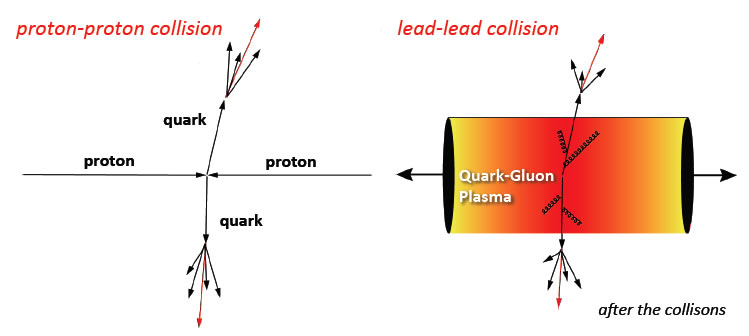
\includegraphics[width=0.7\textwidth]{Chapters/pQCD/collisions.jpg}
 \caption{A schematic approach to a hard partonic interaction in
   (left) a proton-proton interaction and (right) a coloured medium.}
 \label{fig:collision}
\end{center}
\end{figure}


Figure~\ref{fig:collision} is here to give a schematic idea of what
happens in the case of the production of two quark jets. Both quarks
are emitted back to back in the initial parton reference frame. If
they are produced close to the QGP boundary, it is likely that one
will escape, while the second one will scatter and interact
strongly with most of the medium, changing significantly the topology:
the away side is completely absorbed, as measured by the STAR
collaboration in gold-gold (AuAu) collisions~\cite{starquenching}, and
presented in Figure~\ref{fig:jet_star}.
\begin{figure}[h]
\begin{center}
  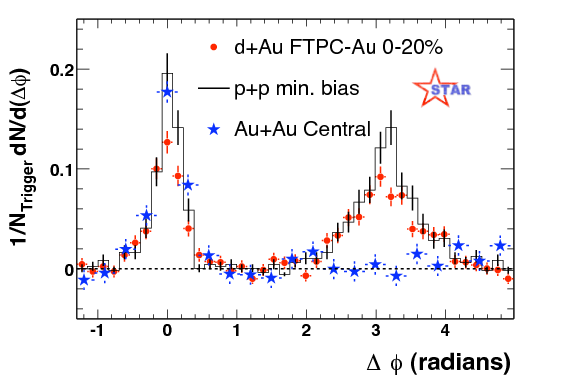
\includegraphics[width=0.7\textwidth]{Chapters/pQCD/jetstar.png}
 \caption{Azimuthal di-hadron correlations in pp (black histogram), dAu (red circles) and AuAu (blue stars) collisions from the STAR collaboration.}
 \label{fig:jet_star}
\end{center}
\end{figure}



On the figure one can see that away-side jets are also slightly modified in
deuteron-gold (dAu) collisions~\cite{starquenching}, indicating some interaction with
non-QGP nuclear matter. Indeed, one does not expect to match the
conditions for a hot medium formation when a very light nucleus (such
as a deuteron) hits a much heavier one. This constitutes a measurement of
nuclear matter effects.

This immediately raises the question of the 'violence' of the QGP
phenomenon. The impact parameter not being measurable, one has to rely
on a model to estimate the \textit{centrality} of the collision.
In various Since the early heavy ion experiments of the seventies and eighties,
the charged hadron multiplicity has been measured to increase
as a function of log $\sqrt{\snn}$, as is shown on Figure~\ref{fig:pbpbmult}. 

\begin{figure}[h]
\begin{center}
  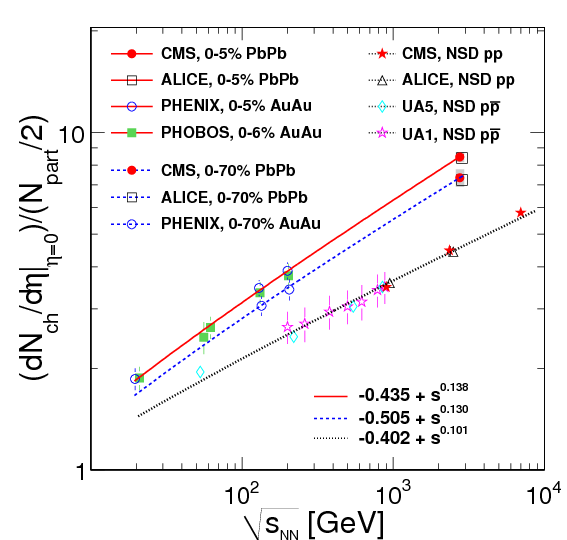
\includegraphics[width=0.6\textwidth]{Chapters/pQCD/multhi.png}
 \caption{Charged hadron multiplicity in proton-proton and heavy ion
   collisions~\cite{pbpbmult}.}
 \label{fig:pbpbmult}
\end{center}
\end{figure}


One
can see that this log $\sqrt{\snn}$ dependence also applies to central
heavy ion collisions. The plot shows that for the most central values, the charged
particle yield changes, as well as the slope, indicating a
classification of events as a function of global event variables works
well. Nowadays the events are cut in percentiles of increasing centrality,
that are directly correlated to the charged hadron multiplicity in the
event or the sum of energy deposits in the forward directions of the
detector.


This short review of possibilities led me to
present the centrality of the collisions, as well as the (p-A or d-A)
baseline for cold nuclear matter effects. This anticipated a
discussion of global event variables which are relevant for any
heavy ion measurement.
In Section~\ref{sec:centrality} I shall present in more detail how
these experimental handles correlate with the assumed number of
nucleons participating in the collisions, as well as with the number
of hard scatterings, both derived from a Glauber model calculation~\cite{Glauber:1970jm}.
% \begin{figure}[h]
% \begin{center}
%   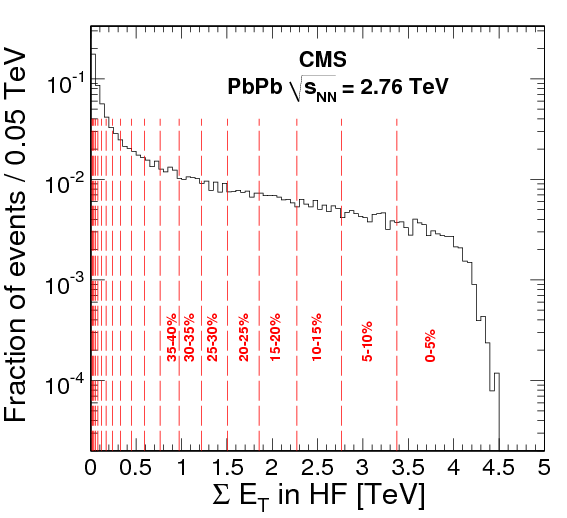
\includegraphics[width=0.6\textwidth]{Chapters/pQCD/centralitybins.png}
%   \includegraphics[width=0.6\textwidth]{Chapters/pQCD/npartncoll.png}
%  \caption{Charged hadron multiplicity in proton-proton and heavy ion collisions}
%  \label{fig:pbpbmult}
% \end{center}
% \end{figure}

Finally, bound states of heavy quarks should play a 
central role in measuring the thermal properties as they also come
from a hard process. Furthermore, the spectroscopy of quarkonia
is such that one family (charmonium or bottomonium) has members with
increasing sizes or binding energy, with different radial and/or orbital quantum numbers. It turns out that
in the most simple considerations, the energy levels computed are of
the order of the deconfinement temperature, or of small integer
multiples of T$_{c}$. This means that \Jpsi, $\psi(2S)$,
\PgU(1S,2S,3S) may react differently to the quark-gluon heat. This is
covered in the next section, in a larger detail.

% All this goes in the positive direction of being able to measure the
% existence of deconfinement in high-energy nuclear reactions. When
% colliding nuclei however, we do not know beforehand if all collisions
% produce a QGP. We can speculate that this depends on the impact
% parameter of each collisions. This is especially important when we
% consider that the geometry of the collision is 
\subsection{Sequential melting}

% Let us take a step back and recall the consequences of asymptotic freedom. As $Q^{2}$
% increases, the coupling decreases, and I have mentioned in Section~\ref{sec:running} that in
% QCD this is due to the existence of gluon self interactions.
%  Probing a colour charge with increasing resolution, one will start to resolve
% more vacuum fluctuations, and by virtue of the colour factors, the
% gluon self couplings play a higher role. In turn, the colour charge
% that one is trying to probe gets \textit{antiscreened} by the gluon
% fields popping out of vacuum.


As seen in Section~\ref{sec:november}, the quarkonium states of the
charmonium family and of the bottomonium family are heavy quark resonances, i.e. a
bound state of heavy quark ($c$ or $b$) and a heavy anti-quark of the
same flavour ($\bar{c}$ or $\bar{b}$, respectively).

Each family has its own spectroscopy, meaning that one can observe
several energy levels of this resonant structure. For example, in the
case of charmonium, the \Jpsi represents the fundamental level of
$c\bar{c}$ states with a spin-parity combination J$^{P}$ =
1$^{-}$. The $\psi(2S)$ state often called ``psi-prime'', is the first radial
excitation of this level. There are other states in the charmonium
family as we shall see in Chapter~\ref{chap:pquarkonia}.


%When thinking about bound states and their radial energy levels, one
%can think about the hydrogen atom, and anticipate that
%higher energy excitations have, as in the Bohr picture, larger radii as
%$n$ increases. Strictly speaking I am not certain how far the analogy
%can be taken, since the hydrogen atom energy levels are function of
%the reduced mass $\mu$ = $m_{p}m_{e}$/$(m_{p}+m_{e})$. Hence in a system
%of two heavy quarks of equal mass, I fear the two-body problem could not be
%easily reduced to a central interaction. But at least the reasoning in
%terms of interaction lengths should hold: a higher energy level seems
%to correspond a wider system.


When studying the effects of the QGP on heavy quark resonances, Matsui
and Satz have found in 1986~\cite{melting} that considering a
non-relativistic interaction potential for two heavy quarks $Q$ and
$\bar{Q}$,
\begin{equation}
\label{eq:potential}
V(r) = \sigma r - \frac{\alpha_{\rm{Coul.}}}{r},
\end{equation}
the string tension $\sigma$ depends on the temperature $T$. For an
isolated system (meaning $T=0$) of charm quarks (let us take for instance the \Jpsi), %they enounce 
we can take $\sigma \approx 1~\GeV/ \textrm{fm}$,
and $\alpha_{\rm{Coul.}} \approx$ 0.5 for the effective Coulomb
interaction coupling. Solving the radial energy equation they get a
\Jpsi radius at zero temperature of

\begin{equation}
E_{\Jpsi} = 3.1 \; \GeV, m_{c} =  1.56 \; \GeV \Longrightarrow r_{\Jpsi} \approx 0.25 \; \,\textrm{fm}.
\end{equation}


The colour screening evolution towards and above QGP transition
temperatures had been studied previously in~\cite{DeGrand}. For a
quark/anti-quark pair, the relevant quantity accounting for a 'size'
is the correlation function $\Gamma_{q\bar{q}}(r,T)$, with $r$ being
the static system's radius, and $T$ the temperature of the gluonic
bath\footnote{At that time, full SU(3) gluons + quarks lattice
  simulation were not available yet.}. From lattice simulations one
can observe the correlation length decreasing steadily when the
temperature passes $T\sim 200$ \MeV. Matsui and Satz identify this with
the binding string tension decreasing with $T$, arguing that at the
deconfinement temperature, $\sigma(T_{c}) = 0$. Above deconfinement
a colour-screened version of the Coulombic potential persists, from
which one can expect dissociation of the quarkonium states at definite
temperature values. In this picture, % speaking of $T_{\rm{diss}}$ or
% energy density is equivalent, and
the resulting physical outcome is a sequential reduction of the overall charmonium yield with increasing
of the energy density created in the collision. 


\begin{figure}[h]
\begin{center}
  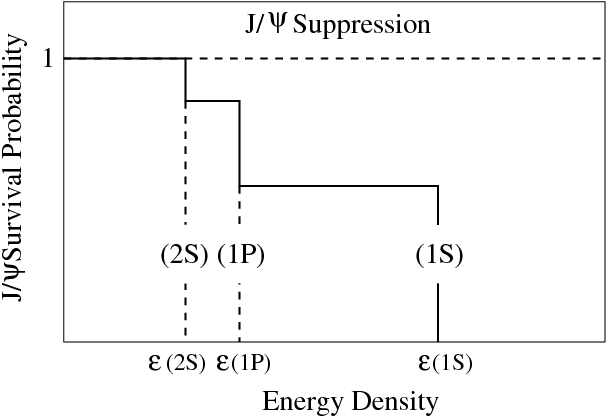
\includegraphics[width=0.5\textwidth]{Chapters/pQCD/seq-charm.png}
  \\ \vspace{1cm}
  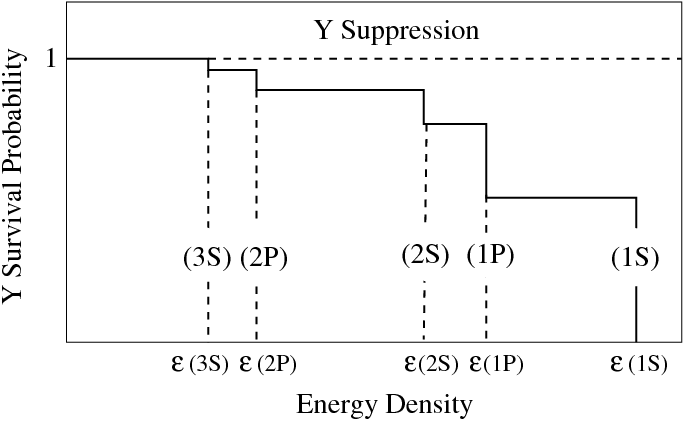
\includegraphics[width=0.5\textwidth]{Chapters/pQCD/seq-bottom.png}
 \caption{A schematic approach to sequential melting of quarkonium
   ground states as a function of energy density. Top: the \Jpsi
   suppression sequence. Bottom: the \PgUa~suppression sequence.}
 \label{fig:sequential}
\end{center}
\end{figure}
\newpage
This is often called a
\textit{sequential melting} scenario, which resembles the rough sketch depicted
in Figure~\ref{fig:sequential}. One can see that the bottomonium
family is slightly more complicated than the charmonium family. I
will elaborate more on the spectroscopies of each family in the next
Chapter. Finally, the height of each step in
Figure~\ref{fig:sequential} is driven by the spectroscopy of each
quarkonium family, where de-excitations from excited levels populate the
lower-lying states.% , and each de-excitation can be assigned a feed-down
% fraction, or probability.


\vspace{0.5em}
\begin{center}
  \fbox{
    \parbox{0.9\textwidth}
    {\textsf {This marks the end of Chapter 1. I have presented how QCD came
together and imposed itself as the theory for strong interactions
between quarks and gluons. I have briefly presented some aspects of what
makes QCD special, and some connections with ultrarelativistic nuclear
collisons in experiments. I have also presented how some observables are
relevant to estimate the effect of the QGP, either in an alteration of
their spectrum, or of their production rate. In the next Chapter I
will concentrate on the case of quarkonia: How do we understand the
production in vacuum of such extended objects, and how we explain
their observed modification in nuclear matter. }}} 
\end{center}



% - Plot de transition de phase QCD ( epsilon/T$^4$ vs T) -> Tc 

% Conclure soit sur une petite liste des signatures (bof), soit sur la mention de Matsui et Satz

% (très facilement connectable avec la température que tu viens d'introduire). 

% Bonus : si t'as envie de mentionner LA mesure de température. 

